% Options for packages loaded elsewhere
\PassOptionsToPackage{unicode}{hyperref}
\PassOptionsToPackage{hyphens}{url}
\PassOptionsToPackage{dvipsnames,svgnames,x11names}{xcolor}
%
\documentclass[
  letterpaper,
  DIV=11,
  numbers=noendperiod]{scrreprt}

\usepackage{amsmath,amssymb}
\usepackage{lmodern}
\usepackage{iftex}
\ifPDFTeX
  \usepackage[T1]{fontenc}
  \usepackage[utf8]{inputenc}
  \usepackage{textcomp} % provide euro and other symbols
\else % if luatex or xetex
  \usepackage{unicode-math}
  \defaultfontfeatures{Scale=MatchLowercase}
  \defaultfontfeatures[\rmfamily]{Ligatures=TeX,Scale=1}
\fi
% Use upquote if available, for straight quotes in verbatim environments
\IfFileExists{upquote.sty}{\usepackage{upquote}}{}
\IfFileExists{microtype.sty}{% use microtype if available
  \usepackage[]{microtype}
  \UseMicrotypeSet[protrusion]{basicmath} % disable protrusion for tt fonts
}{}
\makeatletter
\@ifundefined{KOMAClassName}{% if non-KOMA class
  \IfFileExists{parskip.sty}{%
    \usepackage{parskip}
  }{% else
    \setlength{\parindent}{0pt}
    \setlength{\parskip}{6pt plus 2pt minus 1pt}}
}{% if KOMA class
  \KOMAoptions{parskip=half}}
\makeatother
\usepackage{xcolor}
\setlength{\emergencystretch}{3em} % prevent overfull lines
\setcounter{secnumdepth}{5}
% Make \paragraph and \subparagraph free-standing
\ifx\paragraph\undefined\else
  \let\oldparagraph\paragraph
  \renewcommand{\paragraph}[1]{\oldparagraph{#1}\mbox{}}
\fi
\ifx\subparagraph\undefined\else
  \let\oldsubparagraph\subparagraph
  \renewcommand{\subparagraph}[1]{\oldsubparagraph{#1}\mbox{}}
\fi


\providecommand{\tightlist}{%
  \setlength{\itemsep}{0pt}\setlength{\parskip}{0pt}}\usepackage{longtable,booktabs,array}
\usepackage{calc} % for calculating minipage widths
% Correct order of tables after \paragraph or \subparagraph
\usepackage{etoolbox}
\makeatletter
\patchcmd\longtable{\par}{\if@noskipsec\mbox{}\fi\par}{}{}
\makeatother
% Allow footnotes in longtable head/foot
\IfFileExists{footnotehyper.sty}{\usepackage{footnotehyper}}{\usepackage{footnote}}
\makesavenoteenv{longtable}
\usepackage{graphicx}
\makeatletter
\def\maxwidth{\ifdim\Gin@nat@width>\linewidth\linewidth\else\Gin@nat@width\fi}
\def\maxheight{\ifdim\Gin@nat@height>\textheight\textheight\else\Gin@nat@height\fi}
\makeatother
% Scale images if necessary, so that they will not overflow the page
% margins by default, and it is still possible to overwrite the defaults
% using explicit options in \includegraphics[width, height, ...]{}
\setkeys{Gin}{width=\maxwidth,height=\maxheight,keepaspectratio}
% Set default figure placement to htbp
\makeatletter
\def\fps@figure{htbp}
\makeatother

\KOMAoption{captions}{tableheading}
\makeatletter
\makeatother
\makeatletter
\@ifpackageloaded{bookmark}{}{\usepackage{bookmark}}
\makeatother
\makeatletter
\@ifpackageloaded{caption}{}{\usepackage{caption}}
\AtBeginDocument{%
\ifdefined\contentsname
  \renewcommand*\contentsname{Table of contents}
\else
  \newcommand\contentsname{Table of contents}
\fi
\ifdefined\listfigurename
  \renewcommand*\listfigurename{List of Figures}
\else
  \newcommand\listfigurename{List of Figures}
\fi
\ifdefined\listtablename
  \renewcommand*\listtablename{List of Tables}
\else
  \newcommand\listtablename{List of Tables}
\fi
\ifdefined\figurename
  \renewcommand*\figurename{Figure}
\else
  \newcommand\figurename{Figure}
\fi
\ifdefined\tablename
  \renewcommand*\tablename{Table}
\else
  \newcommand\tablename{Table}
\fi
}
\@ifpackageloaded{float}{}{\usepackage{float}}
\floatstyle{ruled}
\@ifundefined{c@chapter}{\newfloat{codelisting}{h}{lop}}{\newfloat{codelisting}{h}{lop}[chapter]}
\floatname{codelisting}{Listing}
\newcommand*\listoflistings{\listof{codelisting}{List of Listings}}
\makeatother
\makeatletter
\@ifpackageloaded{caption}{}{\usepackage{caption}}
\@ifpackageloaded{subcaption}{}{\usepackage{subcaption}}
\makeatother
\makeatletter
\@ifpackageloaded{tcolorbox}{}{\usepackage[many]{tcolorbox}}
\makeatother
\makeatletter
\@ifundefined{shadecolor}{\definecolor{shadecolor}{rgb}{.97, .97, .97}}
\makeatother
\makeatletter
\makeatother
\ifLuaTeX
  \usepackage{selnolig}  % disable illegal ligatures
\fi
\IfFileExists{bookmark.sty}{\usepackage{bookmark}}{\usepackage{hyperref}}
\IfFileExists{xurl.sty}{\usepackage{xurl}}{} % add URL line breaks if available
\urlstyle{same} % disable monospaced font for URLs
\hypersetup{
  pdftitle={Personal Notes},
  pdfauthor={Ryan Kingery},
  colorlinks=true,
  linkcolor={blue},
  filecolor={Maroon},
  citecolor={Blue},
  urlcolor={Blue},
  pdfcreator={LaTeX via pandoc}}

\title{Personal Notes}
\author{Ryan Kingery}
\date{}

\begin{document}
\maketitle
\ifdefined\Shaded\renewenvironment{Shaded}{\begin{tcolorbox}[enhanced, borderline west={3pt}{0pt}{shadecolor}, breakable, sharp corners, interior hidden, boxrule=0pt, frame hidden]}{\end{tcolorbox}}\fi

\renewcommand*\contentsname{Table of contents}
{
\hypersetup{linkcolor=}
\setcounter{tocdepth}{2}
\tableofcontents
}
\bookmarksetup{startatroot}

\hypertarget{preface}{%
\chapter*{Preface}\label{preface}}
\addcontentsline{toc}{chapter}{Preface}

\markboth{Preface}{Preface}

This page contains notes I've taken over time for several different
subjects of interest. Currently these subjects include

\begin{itemize}
\tightlist
\item
  Classical Mechanics
\item
  Electrodynamics
\item
  Circuit Analysis
\item
  Quantum Mechanics
\item
  Statistical Mechanics
\end{itemize}

Feel free to use whatever you find helpful.

\part{Classical Mechanics}

\hypertarget{newtonian-mechanics}{%
\chapter{Newtonian Mechanics}\label{newtonian-mechanics}}

\textbf{Classical Mechanics} can be thought of as the branch of physics
that focuses on studying the mechanical properties of physical systems
using classical laws. By \emph{mechanical}, we mean we're focused on
analyzing how objects behave in response to \emph{forces}.

By \emph{classical}, we mean we're limiting ourselves to objects that
are neither too big nor too small, and aren't moving too fast. Roughly
speaking, this means the size of objects are between the size of a human
cell to the size of a galaxy cluster, and that those objects aren't
moving anywhere near close to the speed of light.

The oldest and most intuitive formulation of classical mechanics is
\textbf{Newton's Laws}. The idea is that objects move because of forces
that act on them. Understanding mechanics in Newton's formulation is
about understanding the underlying forces, as well as derived quantities
like momentum, torque, and energy.

\hypertarget{point-particles}{%
\section{Point Particles}\label{point-particles}}

In nature, an object is made of matter. It can be composed of many
different molecules arranged in intricate and complicated ways. Further,
each molecule is itself made of atoms, and each atom is itself made up
of subatomic particles. Trying to model the motion of an object would be
extremely cumbersome if we insisted on modeling the dynamics of each
subatomic particle.

Instead, it's convenient to make abstractions. The most convenient
abstraction to make is that we can describe the global behavior of an
object as if it were a point object with no width. It can't spin or
deform. It's one indivisible thing. We call these \textbf{point
particles}.

We'll think of a point particle as following some trajectory in the
3-dimensional Euclidean space \(\mathbb{R}^{3}\). The trajectory or
\textbf{position} is a time-dependent vector

\[
\mathbf{x}(t) = x(t)\mathbf{e}_x + y(t)\mathbf{e}_y + z(t)\mathbf{e}_z.
\] A moving particle also has associated to it a \textbf{velocity}
vector given by

\[
\mathbf{v} = \mathbf{\dot x} = \frac{d\mathbf{x}}{dt}.
\] Perhaps the most fundamental goal of classical mechanics is to find
these two vectors as a function of time. In the Newtonian formulation,
if we want to find a particle's trajectory, we start with the particle's
\textbf{acceleration} vector \[
\mathbf{a} = \mathbf{\dot v} = \mathbf{\ddot x} = \frac{d^2\mathbf{x}}{dt^2},
\] and match it with the \textbf{force} vector \(\mathbf{F}\) via
Newton's Second Law to get a second-order differential equation for
\(\mathbf{x}(t)\).

\hypertarget{newtons-laws}{%
\section{Newton's Laws}\label{newtons-laws}}

Newton's Laws efficiently encapsulate the fundamental physics of
classical mechanics. They're stated below specifically for a point
particle, or \emph{body}, but can be extended to more complex systems as
well.

\begin{enumerate}
\def\labelenumi{\arabic{enumi}.}
\item
  A body remains at rest, or in motion at a constant speed in a straight
  line, unless acted upon by a force. That is,\\
  \[
  \mathbf{F} = \mathbf{0} \Rightarrow \mathbf{v}=const.
  \]
\item
  When a body is acted upon by a force, the time rate of change of its
  acceleration is proportional to the force. That is, \[
  \mathbf{F} = m \mathbf{a}.
  \]
\item
  If two bodies exert forces on each other, these forces have the same
  magnitude but opposite directions. That is, \[
  \mathbf{F}_{12} = \mathbf{F}_{21}.
  \]

  \begin{figure}

  {\centering 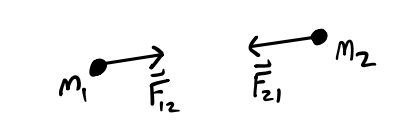
\includegraphics[width=3.125in,height=\textheight]{classical-mechanics/./resources/image-20230212035902274.png}

  }

  \end{figure}
\end{enumerate}

Forces are \textbf{vectors}, which means they obey the superposition
principle, and can be analyzed in components. Position, velocity, and
acceleration are vectors as well. The proportionality constant between
\(\mathbf{F}\) and \(\mathbf{a}\) is called the \textbf{mass }\(m\).
Loosely speaking, the mass of an object is a measure of its
\emph{inertia} or resistance to motion.

The functional form of the forces themselves depend on the particular
type of forces applied. Some common forces are:

\begin{itemize}
\item
  Gravitational Force: \(\mathbf{F} = -\frac{GMm}{r^2} \mathbf{e}_r\)
\item
  Coulomb Force: \(\mathbf{F} = k_e \frac{Qq}{r^2} \mathbf{e}_r\)
\item
  Harmonic Oscillator: \(\mathbf{F} = -k\mathbf{x}\)
\item
  Lorentz Force:
  \(\mathbf{F} = q\mathbf{E} + \frac{q}{c}\mathbf{v} \times \mathbf{B}\)
\item
  Thrust: \(\mathbf{F} = - |\mathbf{v}_{ex}| \dot m \mathbf{e}_v\)

  \begin{figure}

  {\centering 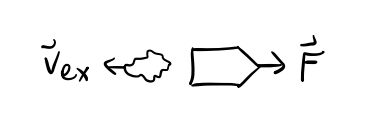
\includegraphics[width=3.125in,height=\textheight]{classical-mechanics/./resources/image-20230212030054782.png}

  }

  \end{figure}
\item
  Normal Forces: \(\mathbf{F} = \mathbf{N}\)
\item
  Tension Forces: \(\mathbf{F} = \mathbf{T}\)
\item
  Frictional Forces: \(\mathbf{F} = -\mu |\mathbf{N}| \mathbf{e}_v\)
\item
  Drag Forces:
  \(\mathbf{F} = -f(\mathbf{v}) \mathbf{e}_v \approx -a\mathbf{v} -b|\mathbf{v}|^2\mathbf{e}_v\)
\item
  Centrifugal Forces:
  \(\mathbf{F} = m\boldsymbol{\omega} \times (\mathbf{x} \times \boldsymbol{\omega})\)
\item
  Coriolis Forces:
  \(\mathbf{F} = 2m \mathbf{v} \times \boldsymbol{\omega}\)
\item
  Buoyant Forces: \(\mathbf{F} = - \rho_{liq} V_{sub} \mathbf{g}\)

  \begin{figure}

  {\centering 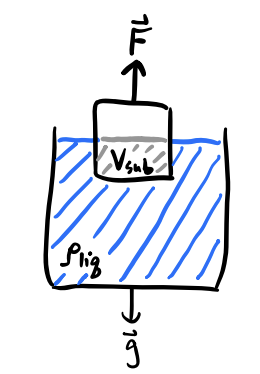
\includegraphics[width=1.5625in,height=\textheight]{classical-mechanics/./resources/image-20230212031757163.png}

  }

  \end{figure}
\end{itemize}

\hypertarget{conservation-laws}{%
\section{Conservation Laws}\label{conservation-laws}}

A quantity Q is said to be \textbf{conserved} if its time derivative is
zero, \(\dot Q = 0\). That is, Q is conserved it it's constant in time.

\hypertarget{momentum}{%
\subsection{Momentum}\label{momentum}}

For an object moving at velocity \(\mathbf{v}\), define its linear
momentum \(\mathbf{p}\) by

\[
\mathbf{p} = m \mathbf{v}.
\] If the mass \(m\) is constant, we evidently have \[
\mathbf{F} = \mathbf{\dot p}.
\] If \(\mathbf{F} = \mathbf{0}\), then \(\mathbf{p}=const\), hence
momentum is conserved if there are no forces applied. This is the
conservation of momentum.

\hypertarget{angular-momentum}{%
\subsection{Angular Momentum}\label{angular-momentum}}

Define the angular momentum \(\mathbf{L}\) of an object by \[
\mathbf{L} = \mathbf{x} \times \mathbf{p}.
\] Similarly, define the \textbf{torque} or \textbf{moment}
\(\mathbf{N}\) by \[\mathbf{N} = \mathbf{x} \times \mathbf{F}.\]

Note both angular momentum and torque depend on the choice of coordinate
system used since the position vector \(\mathbf{x}\) depends on choice
of origin. Now, observe that \[
\mathbf{\dot L} = \mathbf{\dot x} \times \mathbf{p} + \mathbf{x} \times \mathbf{\dot p} = m \mathbf{v} \times \mathbf{v} + \mathbf{x} \times \mathbf{F} = \mathbf{N}.
\] Thus, \(\mathbf{N} = \mathbf{\dot L}\). If
\(\mathbf{N} = \mathbf{0}\), then \(\mathbf{L}=const\), hence angular
momentum must be conserved if there are no torques applied. This is the
conservation of angular momentum.

\hypertarget{work-and-energy}{%
\subsection{Work and Energy}\label{work-and-energy}}

Define the \textbf{work} done \emph{on} an object as it moves along a
path \(\gamma\) from \(A\) to \(B\) by \[
W = \int_A^B \mathbf{F} \cdot d\mathbf{x}.
\]
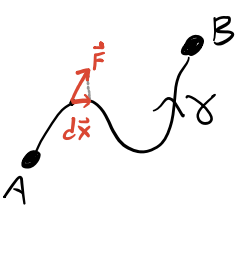
\includegraphics[width=2.08333in,height=\textheight]{classical-mechanics/./resources/image-20230212032859080.png}

In general, work depends on the path taken to get from \(A\) to \(B\),
hence it isn't a unique property of the system.

Observe that \[
dW = \mathbf{F} \cdot d\mathbf{x} = \mathbf{F} \cdot \mathbf{v} dt = d\bigg(\frac{1}{2}m\mathbf{v}^2 \bigg).
\] Define the \textbf{kinetic energy} of the system by
\(T = \frac{1}{2} m \mathbf{v}^2\). Then we evidently have \(dW=dT\).
That is, the work done on the system to get from \(A\) to \(B\) via
\(\gamma\) is just the change in kinetic energy between \(A\) and \(B\),
\[
W = \Delta T = T_B - T_A.
\] When the work done is independent of the path taken it's a state
function of the kinetic energy. In this case, the force \(\mathbf{F}\)
is said to be \textbf{conservative}.

By the Helmholtz theorem, the following conditions are all equivalent:

\begin{itemize}
\tightlist
\item
  \(\mathbf{F}\) is conservative,
\item
  \(W\) is path-independent,
\item
  \(\nabla \times \mathbf{F} = \mathbf{0}\),
\item
  There is a scalar potential \(V=V(\mathbf{x})\) such that
  \(\mathbf{F} = -\nabla V\).
\end{itemize}

The scalar potential \(V\) is called the \textbf{potential energy} of
the system. Evidently, if \(\mathbf{F}\) is conservative, we have \[
W = \int_A^B \mathbf{F} \cdot d\mathbf{x} = -\int_A^B \nabla V \cdot d\mathbf{x} = -\int_A^B dV = V_A - V_B = -\Delta V = \Delta T.
\] That is, \(\Delta T + \Delta V = 0\). Define the total mechanical
\textbf{energy} \(E\) of the system by \[
E = T + V.
\] Then \(\Delta E = \Delta (T + V) = 0\). That is, energy is conserved
when the forces on the system are conservative. This is the conservation
of energy.

Energy isn't generally conserved if the forces aren't conservative.
Examples of non-conservative forces include any force that's a function
of velocity. These include dissipative forces like friction or drag, as
well as magnetic forces.

\hypertarget{examples}{%
\section{Examples}\label{examples}}

The primary goal of mechanics is to understand how systems evolve with
time. To understand a particle's given trajectory in Newtonian
Mechanics, we need to

\begin{itemize}
\tightlist
\item
  Write down all the forces acting on the particle,
\item
  Use \(\mathbf{F} = m \mathbf{a}\) to set up the equations of motion,
\item
  Solve the equations of motion for the trajectory \(\mathbf{x}(t)\),
  either analytically or (usually) numerically.
\end{itemize}

Here are some examples.

\hypertarget{example-projectile-motion}{%
\subsection{Example: Projectile
motion}\label{example-projectile-motion}}

Suppose a cannon is launched from the origin at an angle \(\theta\)
above the ground with initial velocity \(\mathbf{v}_0\).

\begin{figure}

{\centering 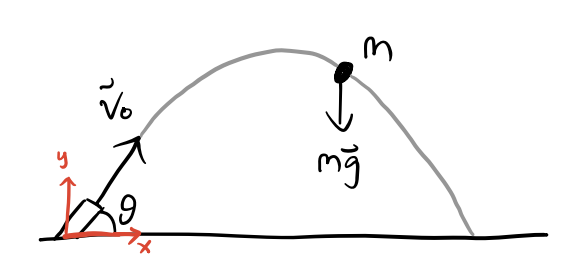
\includegraphics[width=4.16667in,height=\textheight]{classical-mechanics/./resources/image-20230212040005693.png}

}

\end{figure}

\begin{itemize}
\item
  Write down the equations of motion. Assume drag is negligible.

  The forces are \(\mathbf{F} = \mathbf{g} = -g\mathbf{e}_y\). Then, \[
  \mathbf{a} = \ddot x\mathbf{e}_x + \ddot y\mathbf{e}_y = -g\mathbf{e}_y \quad \Longrightarrow \quad   \ddot x = 0, \ \ \ddot y = -mg.
  \]
\item
  Find the trajectory
  \(\mathbf{x}(t) = x(t)\mathbf{e}_x + y(t)\mathbf{e}_y\).

  Integrating each element twice gives \[
  \begin{align*}
  x(t) &= x_0 + v_{0x}t = v_0t \cos \theta, \\
  y(t) &= y_0 + v_{0y}t - \frac{1}{2} gt^2 = v_{0}t\sin \theta - \frac{1}{2} gt^2.
  \end{align*}
  \]
\item
  Find the range, i.e.~the value \(R=x(T)\) when the cannon hits the
  ground. Which launch angle maximizes the range?

  First, we need to find the time \(T\) when \(y(T) = 0\). Setting \[
  y(T) = 0 = v_0 T \sin \theta - \frac{1}{2} gT^2 \Longrightarrow T = 0, \frac{2v_0 \sin \theta}{g}.
  \] The \(T=0\) case is trivial. Plugging the other one in to \(x(T)\)
  finally gives the range, \[
  R = x(T) = v_0T \cos \theta = \frac{2v_0^2 \sin \theta}{g} \cos \theta = \frac{v_0^2 \sin 2\theta}{g}.
  \] Note that the range is maximized when \(\sin 2 \theta = 1\), which
  is when the launch angle is \(\theta = 45^\circ\).
\item
  Find the shape of the motion \(y = y(x)\).

  We need to eliminate \(t\) in both equations and solve for
  \(y=y(x(t))\). Solving \(x(t)\) for \(t\) gives, \[
  x = v_0 t\cos \theta \Longrightarrow t = \frac{x}{v_0 \cos \theta}.
  \] Plugging this into \(y\) then gives \[
  y = v_{0}\frac{x}{v_0 \cos \theta}\sin \theta - \frac{1}{2} g\bigg(\frac{x}{v_0 \cos \theta}\bigg)^2 =  \tan \theta \cdot x - \frac{g}{2v_0^2 \cos^2 \theta} x^2.
  \] This is a downward sloping parabola with vertex at
  \(\big(\frac{v_0^2 \sin 2\theta}{2g}, \frac{v_0^2 \sin^2 \theta}{g}\big)\).
\item
  Find any conserved quantities.

  \begin{itemize}
  \tightlist
  \item
    Momentum: Since \(\mathbf{F} \neq \mathbf{0}\), momentum isn't
    conserved. However, \(p_x\) \emph{is} conserved.
  \item
    Angular Momentum: Since
    \(\mathbf{N} = \mathbf{x} \times \mathbf{F} = \mathbf{x} \times m\mathbf{g} \neq 0\),
    angular momentum is not conserved.
  \item
    Energy: Since \(V=mgy\), the force \(\mathbf{F}\) is conservative,
    hence energy is conserved.
  \end{itemize}
\end{itemize}

\hypertarget{example-block-sliding-on-a-ramp-with-friction}{%
\subsection{Example: Block sliding on a ramp with
friction}\label{example-block-sliding-on-a-ramp-with-friction}}

A block of mass \(m\) is sliding down a ramp inclined from the
horizontal at an angle \(\theta\). Assume the system has a coefficient
of friction \(\mu\), and that the block starts from rest at the top of
the ramp.

\begin{figure}

{\centering 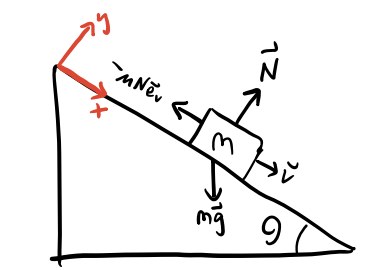
\includegraphics[width=3.64583in,height=\textheight]{classical-mechanics/./resources/image-20230212033443698.png}

}

\end{figure}

\begin{itemize}
\item
  Write down the equations of motion.

  Choose a coordinate system such that \(x\) is pointing downwards
  parallel to the ramp and \(y\) is pointing outwards perpendicular to
  the ramp. There are three forces acting, gravity, the normal force,
  and the frictional force, so \[
  \mathbf{F} = \mathbf{N} + m\mathbf{g} - \mu \mathbf{N} \mathbf{e}_v = N\mathbf{e}_y + mg(\sin\theta\mathbf{e}_x - \cos\theta\mathbf{e}_y) - \mu N \mathbf{e}_x.
  \] Resolving into components, we have \[
  \begin{align*} 
  m \ddot x &= mg\sin\theta - \mu N, \\
  m \ddot y &= N - mg\cos\theta = 0.
  \end{align*}
  \] The second equation follows from the assumption that the block is
  constrained to stay on the ramp.
\item
  Find the trajectory
  \(\mathbf{x}(t) = x(t)\mathbf{e}_x + y(t)\mathbf{e}_y\).

  To solve, we need to eliminate the normal force \(N\). Using the EOM
  for \(\ddot y\), we get \(N = mg\cos\theta\). Plugging this into the
  equation for \(\ddot x\) then gives

  \[
  \begin{align*} 
  \ddot x &= g(\sin\theta - \mu\cos\theta) = const, \\
  \ddot y &= 0.
  \end{align*}
  \] Suppose the block starts at the top of the ramp, which we'll call
  the origin. Then integrating, we get,

  \[
  \begin{align*} 
  x(t) &= v_0 t + \frac{1}{2}g(\sin\theta - \mu\cos\theta)t^2, \\
  y(t) &= 0.
  \end{align*}
  \] Notice \(x(t)\) is just the equation of an object falling under a
  modified gravity \[
  \mathbf{g}'=-g(\sin\theta - \mu\cos\theta)\mathbf{e}_x.
  \]
\item
  Find the angle \(\theta\) at which the block will start sliding.

  The block will move if \(\ddot x \geq 0\), i.e.~when
  \(\mu \leq \tan\theta\). It will start moving at the angle when
  \(\tan\theta=\mu\) exactly, i.e.~when \[
  \theta = \arctan\mu.
  \]
\item
  Find any conserved quantities.

  \begin{itemize}
  \tightlist
  \item
    Momentum: Since \(\mathbf{F} \neq \mathbf{0}\), momentum is not
    conserved. However, \(p_y\) is conserved.
  \item
    Angular momentum: Since
    \(\mathbf{N} = \mathbf{x} \times \mathbf{F} \neq \mathbf{0}\),
    angular momentum is not conserved.
  \item
    Energy: Since friction is present, \(\mathbf{F}\) is a dissipative
    force, hence it's not conservative, and energy is not conserved.
  \end{itemize}
\item
  Find the rate of energy dissipation as the block slides down the ramp.

  Friction dissipates as a heat \(Q\). If the block slides a distance
  \(L\), this means \(E(0) = E(L) + Q\). Since the block starts from
  rest, \(E(0) = 0\). At \(x=L\), the work done is \[
  W = \int_0^L F_x dx = \int_0^L mg(\sin\theta - \mu\cos\theta)dx = mgL(\sin\theta - \mu\cos\theta) = T(L) - 0 = T(L),
  \] so the energy when the block gets to the bottom is \[
  E(L) = T(L) + V(L,0) = mgL(\sin\theta - \mu\cos\theta) - mgL\sin\theta = -\mu mgL\cos\theta.
  \] Finally, using this to solve for \(Q\), the heat dissipated over
  the entire trajectory, we get \[
  Q = E(0) - E(L) = \mu mgL\cos\theta.
  \] The most important sanity check here is to notice there's no heat
  dissipation if there is no friction.
\end{itemize}

\hypertarget{curvilinear-coordinates}{%
\section{Curvilinear Coordinates}\label{curvilinear-coordinates}}

For many problems, it's more convenient to take advantage of the
underlying symmetry by using special coordinate systems. Other than
rectangular coordinates \((x,y,z)\), the most common coordinate systems
worth being familiar with are polar coordinates \((r,\varphi)\),
cylindrical coordinates \((\rho,\varphi,z)\), and spherical coordinates
\((r,\theta,\varphi)\).

\hypertarget{polar-coordinates}{%
\subsection{Polar Coordinates}\label{polar-coordinates}}

For problems with circular symmetry it's convenient to use polar
coordinates \((r,\varphi)\), defined by

\[
\begin{align*} 
x &=  r\cos\varphi, \\ 
y &=  r\sin\varphi. \\
\end{align*}
\] where \(r \geq 0\) and \(0 \leq \varphi \leq 2\pi\). We can assign
basis vectors to polar coordinates \(\mathbf{e}_r, \mathbf{e}_\varphi\)
to each point as usual.

\begin{figure}

{\centering 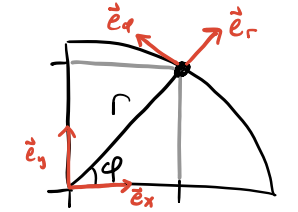
\includegraphics[width=3.125in,height=\textheight]{classical-mechanics/./resources/image-20230212040057533.png}

}

\end{figure}

The thing to keep in mind is that these curvilinear basis vectors are
now functions of position,

\[
\begin{align*} 
\mathbf{e}_r &= \mathbf{e}_r(r, \varphi), \\ 
\mathbf{e}_\varphi &= \mathbf{e}_\varphi(r, \varphi). 
\end{align*}
\] We can figure out how these basis vectors change by taking their
differentials, which follow from the figure above,

\[
\begin{align*} 
d\mathbf{e}_r &= \mathbf{e}_\varphi d\varphi, \\ 
d\mathbf{e}_\varphi &= -\mathbf{e}_r d\varphi.
\end{align*}
\] Using these differential forms, we can conclude that the motion
vectors change as follows,

\[
\begin{align*}
\mathbf{x} &= r\mathbf{e}_r, \\
\mathbf{v} &= \dot r \mathbf{e}_r + r\dot \varphi \mathbf{e}_\varphi, \\
\mathbf{a} &= (\ddot r - r\dot \varphi^2)\mathbf{e}_r + (2\dot r \dot \varphi + r\ddot \varphi)\mathbf{e}_\varphi.
\end{align*}
\]

\hypertarget{example-circular-orbits}{%
\subsection{Example: Circular orbits}\label{example-circular-orbits}}

Suppose an object moves in a circular orbit of radius \(r\) at a
constant angular velocity \(\omega\) due to a central force
\(\mathbf{F} = -F\mathbf{e}_r\).

\begin{figure}

{\centering 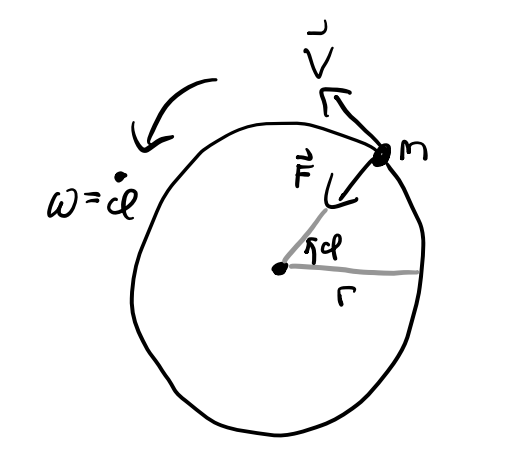
\includegraphics[width=3.125in,height=\textheight]{classical-mechanics/./resources/image-20230212033719862.png}

}

\end{figure}

\begin{itemize}
\item
  Find the equations of motion. Since the object moves at constant
  \(\omega\), we have \(\dot \varphi = \omega = const\). Using the polar
  equations for velocity and acceleration, we have \[
  \begin{align*}
  \mathbf{v} &= \dot r \mathbf{e}_r, \\
  \mathbf{a} &= -r\omega^2\mathbf{e}_r + r \dot \omega\mathbf{e}_\varphi = - \frac{F}{m}\mathbf{e}_r.
  \end{align*}
  \] Note we can re-write these equations to get \(F = m\omega^2 r\).
\item
  Find the \emph{period} \(\tau\) of the orbit.

  We want the time it takes for \(\Delta \varphi = 2\pi\). Since
  \(\Delta \varphi = \omega\tau\), solving for \(\tau\) gives
  \[\tau = \frac{2\pi}{\omega}.\]
\item
  Suppose the central force is the gravitational force,
  \(F = \frac{GMm}{r^2}\). Find the angular velocity, the period, and
  the orbital velocity as a function of \(G, M, r\).

  We have \[
  F = \frac{GMm}{r^2} = m\omega^2 r \ \Longrightarrow \ \omega = \sqrt{\frac{GM}{r^3}} \ \Longrightarrow \ \tau = \frac{2\pi}{\sqrt{GM}} r^{3/2}.
  \] This is just a special case of Kepler's third law,
  \(\tau^2 \propto r^3\). The orbital velocity is given by \[
  v = r\omega = \sqrt{\frac{GM}{r}}.
  \]
\end{itemize}

\hypertarget{example-simple-pendulum}{%
\subsection{Example: Simple pendulum}\label{example-simple-pendulum}}

Consider the problem of the simple pendulum, where a mass \(m\) swings
on a massless string of length \(\ell\) under the force of gravity. The
string is fixed at one point. Assume no damping is present.

\begin{figure}

{\centering 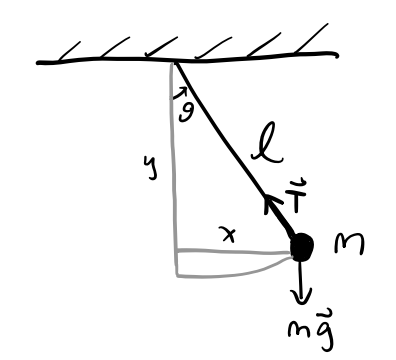
\includegraphics[width=3.125in,height=\textheight]{classical-mechanics/./resources/image-20230212040128210.png}

}

\end{figure}

\begin{itemize}
\item
  Find the equations of motion from the forces directly.

  There are two forces in this problem, gravity and the tension in the
  string, \[
  \mathbf{F} = \mathbf{T} + m\mathbf{g} = -T\mathbf{e}_r + mg(\cos\theta \mathbf{e}_r - \sin\theta\mathbf{e}_\theta).
  \] Dividing by \(m\) and setting equal to the polar form of
  \(\mathbf{a}\), we have \[
  \mathbf{a} = (-T+mg\cos\theta)\mathbf{e}_r - mg\sin\theta\mathbf{e}_\theta = -m\ell^2 \dot \theta^2 \mathbf{e}_r + m\ell^2 \ddot \theta \mathbf{e}_\theta.
  \] This gives two equations of motion, one for the tension and one for
  the angular acceleration, \[
  \begin{align*}
  T &= m\ell^2 \dot\theta^2 + mg\cos\theta, \\
  \ddot \theta &= -\frac{g}{\ell} \sin\theta. \\
  \end{align*}
  \]
\item
  Find the equations of motion again, but this time using torques.

  Recall \(\mathbf{N} = I \boldsymbol{\dot \omega}\), where \(I\) is the
  scalar moment of inertia and \(\boldsymbol{\omega}\) is the angular
  velocity vector. In this case, \(I=m\ell^2\) and
  \(\boldsymbol{\dot \omega} = \ddot \theta \mathbf{e}_z\). Then we have
  \[
  I \boldsymbol{\dot \omega} = m\ell^2 \ddot \theta \mathbf{e}_z \equiv \ell\mathbf{e}_r \times m\mathbf{g} = -mg\ell\sin\theta \mathbf{e}_z = \mathbf{N},
  \] which can be solve to get
  \(\ddot \theta = -\frac{g}{\ell}\sin\theta\). Notice how in this
  approach we don't need to worry about the tension at all.
\item
  Suppose \(\theta\) is small. Write down the equations of motion, solve
  them, and find the period.

  When \(\theta \ll 1\) the small angle approximation applies,
  \(\sin\theta \approx \theta\). In this case, the equation of motion
  reduces to \[\ddot \theta = -\frac{g}{\ell} \theta,\] which is just
  simple harmonic oscillation with angular frequency
  \(\omega = \sqrt{\frac{g}{\ell}}\). The solution to SHO is \[
  \theta(t) = A\sin(\omega t + \phi),
  \] where \(A\) is some amplitude and \(\phi\) is some phase determined
  by the initial conditions. Finally, solving for the period, we have \[
  \tau = \frac{2\pi}{\omega} = 2\pi\sqrt{\frac{\ell}{g}}.
  \]
\end{itemize}

\hypertarget{cylindrical-coordinates}{%
\subsection{Cylindrical Coordinates}\label{cylindrical-coordinates}}

Cylindrical coordinates extend polar coodinates by adding in the z-axis
from the rectangular system,

\[
\begin{align*} 
x &=  r\cos\varphi, \\ 
y &=  r\sin\varphi, \\
z &= z.
\end{align*}
\] The basis vectors are
\(\mathbf{e}_r, \mathbf{e}_\varphi, \mathbf{e}_z\). Their differential
forms are just \[
\begin{align*} 
d\mathbf{e}_r &= \mathbf{e}_\varphi d\varphi, \\ 
d\mathbf{e}_\varphi &= -\mathbf{e}_r d\varphi \\ 
d\mathbf{e}_z &= 0. 
\end{align*}
\] The motion vectors in cylindrical coordinates are thus given by, \[
\begin{align*}
\mathbf{x} &= r\mathbf{e}_r, \\
\mathbf{v} &= \dot r \mathbf{e}_r + r\dot \varphi \mathbf{e}_\varphi + \dot z \mathbf{e}_z , \\
\mathbf{a} &= (\ddot r - r\dot \varphi^2)\mathbf{e}_r + (2\dot r \dot \varphi + r\ddot \varphi)\mathbf{e}_\varphi + \ddot z \mathbf{e}_z.
\end{align*}
\]

\hypertarget{spherical-coordinates}{%
\subsection{Spherical Coordinates}\label{spherical-coordinates}}

Spherical coordinates extend polar coordinates in a slightly different
way. The radius \(r\) is now 3-dimensional, and there are two angles, a
\emph{polar angle} \(0 \leq \theta \leq \pi\) and an \emph{azimuthal
angle} \(0 \leq \varphi \leq 2\pi\). The conversion to rectangular
coordinates is given by, \[
\begin{align*} 
x &=  r\sin\theta\cos\varphi, \\ 
y &=  r\sin\theta\sin\varphi, \\
z &= r\cos\theta. \\ 
\end{align*}
\] The basis vectors are
\(\mathbf{e}_r, \mathbf{e}_\theta, \mathbf{e}_\varphi\). Deriving the
differential forms of these is a good bit more complex. Here they are,
\[
\begin{aligned}
d\mathbf{e}_r &= \dot\theta \sin\varphi d\mathbf{e}_\theta + \dot\varphi d\mathbf{e}_\varphi, \\
d\mathbf{e}_\theta &= - \dot\theta \sin\varphi d\mathbf{e}_r - \dot\theta \cos\varphi d\mathbf{e}_\varphi, \\
d\mathbf{e}_\varphi &= - \dot\varphi \mathbf{e}_r + \dot\theta \cos\varphi \mathbf{e}_\theta. \\
\end{aligned}
\] These can then be used to get the motion vectors in spherical
coordinates, \[
\begin{align*}
\mathbf{r} &= r \mathbf{e}_r, \\
\mathbf{v} &= \dot{r} \mathbf{e}_r + r \dot\theta \sin\varphi \mathbf{e}_{\theta} + r \dot\varphi \mathbf{e}_{\varphi}, \\
\mathbf{a} &= (\ddot{r} - r \dot{\theta}^2 \sin^2\varphi - r \dot{\varphi}^2) \mathbf{e}_r \\
&\quad + (r \ddot\theta \sin\varphi + 2 \dot{r} \dot\theta \sin\varphi + 2 r \dot\theta \dot\varphi \cos\varphi) \mathbf{e}_{\theta} \\
&\quad + (r \ddot\varphi + 2 \dot{r} \dot\varphi - r \dot{\theta}^2 \sin\varphi \cos\varphi) \mathbf{e}_{\varphi}. \\
\end{align*}
\]

\hypertarget{many-particle-systems}{%
\section{Many-Particle Systems}\label{many-particle-systems}}

Thus far we've worked with single-particle systems. Let's now consider a
system of \(N\) particles with positions
\(\mathbf{x}_1, \mathbf{x}_2, \cdots, \mathbf{x}_N\) respectively. We
can use the principle of superposition to extend the laws derived above
for single particles.

For \(N\)-particle systems it's convenient to characterize the system's
position using the \textbf{center of mass} vector \(\mathbf{R}\), \[
\mathbf{R} \equiv \frac{1}{M}\sum_{i=1}^N m_i \mathbf{x}_i,
\] where \(M\) is just the \emph{total mass} of the system,
\(M \equiv \sum m_i\). The center of mass is just the mass-weighted
average of all the particle position vectors.

Suppose an external force \(\mathbf{F}^{ext}\) is acting on the system,
and suppose each particle \(i\) imparts a force \(\mathbf{F}_{ij}\) on
particle \(j \neq i\). Here's what this would look like for \(N=3\)
particles.

\begin{figure}

{\centering 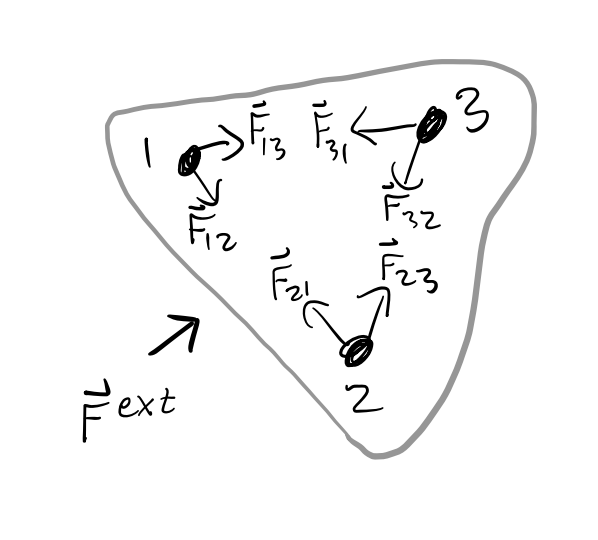
\includegraphics[width=3.125in,height=\textheight]{classical-mechanics/./resources/image-20230212034236830.png}

}

\end{figure}

By superposition, the total force acting on the entire system is thus,
\[
\mathbf{F} = \mathbf{F}^{ext} + \sum_{i \neq j} \mathbf{F}_{ij} = \sum m_i \mathbf{a}_i = M\mathbf{\ddot R}.
\] Now, by Newton's third law, \(\mathbf{F}_{ij} = -\mathbf{F}_{ji}\).
This means all the internal forces cancel in pairs, so we have \[
\mathbf{F}^{ext} = M\mathbf{\ddot R}.
\] That is, the system as a whole moves as if it were a point mass \(M\)
with an external force \(\mathbf{F}^{ext}\) acting on its center of mass
\(\mathbf{R}\).

If the total momentum is defined as \(\mathbf{P} = M \mathbf{\dot R}\),
this expression then says \(\mathbf{F}^{ext} = \mathbf{\dot P}\). Thus,
if no external forces act on the system, then its total linear momentum
\(\mathbf{P}\) is conserved.

Let's now consider the total \emph{torques} on the system. Suppose the
system experiences an external torque \(\mathbf{N}^{ext}\), and that
each particle \(i\) exerts a torque \(\mathbf{N}_{ij}\) on particle
\(j\). Then by superposition, the total torque on the system is \[
\mathbf{N} = \mathbf{N}^{ext} + \sum_{i \neq j} \mathbf{N}_{ij} = \mathbf{N}^{ext} + \sum_{i \neq j} \mathbf{x}_i \times \mathbf{F}_{ij},
\] Again, we can use the fact that each
\(\mathbf{F}_{ij} = -\mathbf{F}_{ji}\). If we do this, we can re-write
the total torque as

\[
\mathbf{N} = \mathbf{N}^{ext} + \sum_{i<j} (\mathbf{x}_{i}-\mathbf{x}_{j}) \times \mathbf{F}_{ij} = \mathbf{N}^{ext}.
\] Now, if we further assume that each internal force acts centrally,
i.e.~\(\mathbf{F}_{ij} = \mathbf{F}_{ij}(\mathbf{x}_{i}-\mathbf{x}_{j})\),
then the internal cross products all vanish, and we just get
\(\mathbf{N} = \mathbf{N}^{ext}\). That is, if all the internal forces
are central, then the total torque on the system is just the external
torque.

If the total angular momentum on the system is defined as
\(\mathbf{L} = \mathbf{R} \times \mathbf{P}\), this expression says
\(\mathbf{\dot L} = \mathbf{N}^{ext}\). Thus, if no external torques act
on the system, then its total angular momentum \(\mathbf{L}\) is
conserved.

It's insightful to separate each particle's motion vectors explicitly
into a center of mass component and a relative component,

\[
\begin{align*} 
\mathbf{x}_i &= \mathbf{R} + \boldsymbol{\mathscr{r}}_i, \\
\mathbf{v}_i &= \mathbf{V} + \boldsymbol{\mathscr{v}}_i. \\
\end{align*}
\]
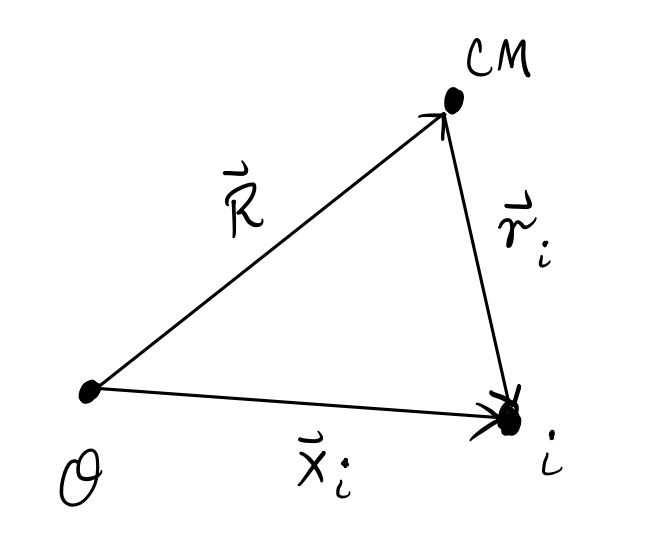
\includegraphics[width=2.08333in,height=\textheight]{classical-mechanics/./resources/image-20230213071525149.png}

Let's re-write the total angular momentum \(\mathbf{L}\) in terms of
these vectors,

\[
\begin{align*} 
\mathbf{L} &= \sum \mathbf{x}_i \times \mathbf{p}_i = \sum (\mathbf{R} + \boldsymbol{\mathscr{r}}_i) \times m_i(\mathbf{V} + \boldsymbol{\mathscr{v}}_i) \\
&= M\mathbf{R} \times \mathbf{V} + \sum m_i \boldsymbol{\mathscr{r}}_i \times \boldsymbol{\mathscr{v}}_i + \mathbf{R} \times \bigg(\sum m_i \boldsymbol{\mathscr{v}}_i \bigg) + \bigg(\sum m_i \boldsymbol{\mathscr{r}}_i \bigg)\times \mathbf{V} \\
&= \mathbf{R} \times \mathbf{P} + \sum m_i \boldsymbol{\mathscr{r}}_i \times \boldsymbol{\mathscr{v}}_i \\
&\equiv \mathbf{L}^{orb} + \mathbf{L}^{spin}. \\
\end{align*}
\] We've thus been able to separate the angular momentum into two
components, an \textbf{orbital angular momentum}
\(\mathbf{L}^{orb} = \mathbf{R} \times \mathbf{P}\), and a \textbf{spin
angular momentum}
\(\mathbf{L}^{spin} = \sum m_i \boldsymbol{\mathscr{r}}_i \times \boldsymbol{\mathscr{v}}_i\).
The orbital angular momentum describes how the center of mass of the
object tends to rotate about some external point. The spin angular
momentum describes how the system itself tends to rotate about its
center of mass.

\begin{figure}

{\centering 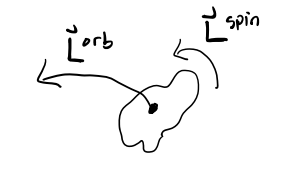
\includegraphics[width=2.08333in,height=\textheight]{classical-mechanics/./resources/image-20230212040206890.png}

}

\end{figure}

Last, let's look at the total energies of the system. For a system with
\(N\) particles, the potential energy will be a function of all the
position vectors,
\(V = V(\mathbf{x}_1, \mathbf{x}_2, \cdots, \mathbf{x}_N)\). It won't
generally simplify. But the kinetic energy we can simplify. Writing it
in terms of its relative and center of mass velocities, we have

\[
\begin{align*}
T &= \frac{1}{2}\sum m_i \mathbf{v}_i^2 = \sum m_i (\mathbf{V} + \boldsymbol{\mathscr{v}}_i)^2 \\
&= \frac{1}{2}M\mathbf{V}^2 + \frac{1}{2}\sum m_i\boldsymbol{\mathscr{v}}_i^2 + \mathbf{V} \cdot \bigg(\sum m_i \boldsymbol{\mathscr{v}}_i\bigg) \\
&= \frac{1}{2}M\mathbf{V}^2 + \frac{1}{2}\sum m_i\boldsymbol{\mathscr{v}}_i^2 \\
&= T^{CM} + T^{rel}.
\end{align*}
\] Thus, the kinetic energy separates into a sum of the kinetic energy
on the center of mass \(T^{CM} = \frac{1}{2}M\mathbf{V}^2\), and the
kinetic energy of the relative components
\(T^{rel} = \frac{1}{2}\sum m_i\boldsymbol{\mathscr{v}}_i^2\).
Evidently, the total energy is \[
E = T + V = T^{CM} + T^{rel} + V(\mathbf{x}_1, \mathbf{x}_2, \cdots, \mathbf{x}_N).
\] It's conserved provided the external force \(\mathbf{F}^{ext}\) is
conservative.

\hypertarget{example-rockets}{%
\subsection{Example: Rockets}\label{example-rockets}}

Suppose a rocket of mass \(m_0=m(t) + m_{ex}(t)\) is moving through free
space with no external forces acting on it. It's expelling fuel for
trust at some constant speed \(v_{ex}\) with respect to the rocket.

\begin{figure}

{\centering 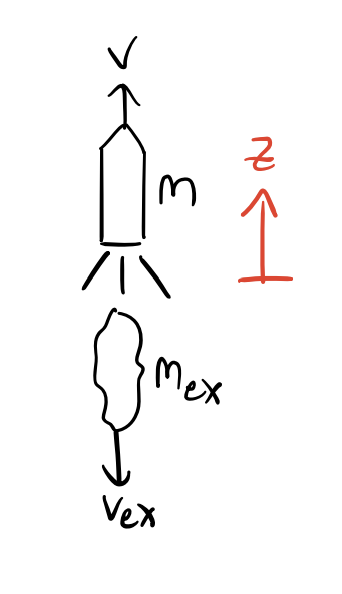
\includegraphics[width=1.5625in,height=\textheight]{classical-mechanics/./resources/image-20230212033930176.png}

}

\end{figure}

\begin{itemize}
\item
  What is the force of thrust on the rocket?

  No external forces are present, so \(\mathbf{F}^{ext} = \mathbf{0}\).
  The internal forces are the thrust of the rocket, and the force of the
  exhaust. In the frame of the rocket they cancel out,
  \(\mathbf{F}_{th} = \mathbf{F}_{ex}\), so we have \[
  \mathbf{F}_{th} = -\mathbf{F}_{ex} = -\mathbf{\dot p}_{ex} = -\frac{d}{dt}(m_{ex} \mathbf{v}_{ex}) = -\dot m_{ex} \mathbf{v}_{ex}.
  \] Now, since \(m_0 = m + m_{ex}\), \(\dot m = -\dot m_{ex}\), and
  \(\mathbf{v}_{ex} = -v_{ex}\mathbf{e}_v\), we have \[
  \mathbf{F}_{th} = -\dot m v_{ex} \mathbf{e}_v.
  \]
\item
  Find the velocity \(\mathbf{v}(t)\) of the rocket.

  Using the fact that \(\mathbf{F}_{th} = m\mathbf{a}\), we have
  \(-\dot m v_{ex} = m \dot v\), a first-order differential equation in
  \(v(t)\), \[
  \dot v + v_{ex} \frac{\dot m}{m} = 0.
  \] Integrating both sides and solving for \(v(t)\), we get \[
  v(t) = v_0 - v_{ex} \int_{m_0}^m \frac{dm}{m} = -v_{ex} \log \frac{m(t)}{m_0}.
  \] Or, expressing in the form of the well-known \emph{rocket
  equation}, \[
  \Delta v = v_{ex} \log\frac{m_0}{m(t)}.
  \]
\item
  Find the position \(\mathbf{x}(t)\) of the rocket, assuming fuel is
  expelled form the rocket at a constant rate.

  Assume \(\dot m = -k = const\). Since there are no external forces,
  the rocket must be traveling along some line. Suppose without loss of
  generality then that \(\mathbf{x}(t) = z(t)\mathbf{e}_z\). Then we
  have, \[
  \begin{align*}
  z(t) &= \int_0^t v(t) dt = v_{ex} \int_0^t dt \log\frac{m_0}{m_0-kt} \\
  &= v_{ex} \bigg[t - \bigg(\frac{m_0-kt}{k} \bigg) \log \bigg(\frac{m_0}{m_0-kt} \bigg) \bigg] \\
  &= v_{ex} t - \frac{v_{ex}}{k}(m_0 - kt)\log\bigg(\frac{m_0}{m_0-kt} \bigg).
  \end{align*}
  \]
\end{itemize}

\hypertarget{simple-systems}{%
\chapter{Simple Systems}\label{simple-systems}}

Even if we can easily find the equations of motion of a system, very few
are simple enough to solve exactly using analytical methods. In this
lesson we'll consider some of the most common such systems. We'll focus
on (possibly non-conservative) forces acting on a single-particle
particle of mass \(m\) that take the form, \[
\mathbf{F} = \mathbf{F}(\mathbf{x}, \mathbf{v}, t).
\] We'll assume \(\mathbf{F}\) is either linear or quadratic in position
and velocity. With a few exceptions, these are the few cases for which
we can even solve the equations of motion analytically.

For the most part, we'll focus on the case when everything is
1-dimensional, \(F = F(x, v, t)\). While we'll speak in this lesson of
\(F\) being a force, \(x\) a position, and \(v\) a velocity, the methods
we describe indeed can apply to many other situations as well.

For example, \(x\) could represent a generalized coordinate (say an
angle), in which case \(v\) would be a generalized velocity (say an
angular velocity) and \(F\) a generalized force (say a torque). In some
cases, \(x\) need not be a coordinate at all. For example, we can use
the same techniques from this lesson to analyze a simple circuit, in
which case \(x\) would be a charge or a current and \(F\) would be a
supplied voltage.

\hypertarget{independent-forces}{%
\section{Independent Forces}\label{independent-forces}}

The first and simplest case we'll consider are forces that don't depend
on position or velocity, \[
m \mathbf{a} = \mathbf{F}_0(t).
\] We can solve these systems directly by integrating both sides,
i.e.~\emph{reducing to quadrature}. We have,

\[
\begin{align*}
\mathbf{a}(t) &= \frac{1}{m}\mathbf{F}_0(t), \\
\mathbf{v}(t) &= \mathbf{v}_0 + \frac{1}{m}\int_0^t dt'\mathbf{F}_0(t'), \\
\mathbf{x}(t) &= \mathbf{x}_0 + \mathbf{v}_0t + \frac{1}{m}\int_0^t dt' \int_0^{t'} dt''\mathbf{F}_0(t''). \\
\end{align*}
\] The simplest of these cases are when there are no forces at all, and
when the forces are constant. If there are no forces at all acting on
the system, \(\mathbf{F}_0 = \mathbf{0}\), in which case the equations
of motion reduce to

\[
\begin{align*}
\mathbf{a}(t) &= 0, \\
\mathbf{v}(t) &= \mathbf{v}_0, \\
\mathbf{x}(t) &= \mathbf{x}_0 + \mathbf{v}_0t. \\
\end{align*}
\] This is just a statement of Newton's First Law. If no forces act on a
particle, it continues linearly along its path at constant velocity. The
next simplest case is when \(\mathbf{F}_0=const\). In this case, the
equations of motion become

\[
\begin{align*}
\mathbf{a}(t) &= \frac{1}{m}\mathbf{F}_0, \\
\mathbf{v}(t) &= \mathbf{v}_0 + \frac{1}{m}\mathbf{F}_0 t, \\
\mathbf{x}(t) &= \mathbf{x}_0 + \mathbf{v}_0t + \frac{1}{2m^2}\mathbf{F}_0^2. \\
\end{align*}
\] This case includes the gravitional force near the surface of the
Earth, in which case \(\mathbf{F}_0=m\mathbf{g}\). It also includes the
problem of an electric charge placed close to a large conducting sheet
with a uniform electric field, where \(\mathbf{F}_0=q\mathbf{E}_0\).

In these problems, the motion will always be along a parabolic arc. The
parabola will slope toward the force if the force is attractive, and
away from the force if it's repulsive.

\hypertarget{example-free-fall-near-earth}{%
\subsection{Example: Free-fall near
Earth}\label{example-free-fall-near-earth}}

Suppose an object of mass \(m\) is falling freely near the Earth's
surface. In this case, \(\mathbf{F}_0 = m\mathbf{g}\), so

\[
\begin{align*}
\mathbf{a}(t) &= \mathbf{g}, \\
\mathbf{v}(t) &= \mathbf{v}_0 - \mathbf{g}t, \\
\mathbf{x}(t) &= \mathbf{x}_0 + \mathbf{v}_0t + \frac{1}{2}\mathbf{g}t^2.
\end{align*}
\] The motion in this case will always lie in the plane spanned by
\(\mathbf{v}_0\) and \(\mathbf{g}\). This means without loss of
generality we can assume motion lies in the xy-plane with
\(\mathbf{g} = -g\mathbf{e}_y\). Then \(y\) can be solved as a function
of \(x\) to give \[
y(x) = v_{0}\frac{x}{v_0 \cos \theta}\sin \theta - \frac{1}{2} g\bigg(\frac{x}{v_0 \cos \theta}\bigg)^2,
\] which is of course a downward-sloping parabola centered at the vertex
\(\big(\frac{v_0^2 \sin 2\theta}{2g}, \frac{v_0^2 \sin^2 \theta}{g}\big)\).

\begin{figure}

{\centering 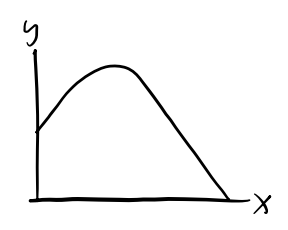
\includegraphics[width=2.08333in,height=\textheight]{classical-mechanics/./resources/image-20230214035909918.png}

}

\end{figure}

\hypertarget{drag-forces}{%
\section{Drag Forces}\label{drag-forces}}

The next type of forces we'll consider are those which are functions of
velocity,

\[
m\mathbf{a} = \mathbf{F}(\mathbf{v}).
\] In the 1-dimensional case, this reduces to,

\[
ma = F(v).
\] Provided \(v\) is small, we can approximate \(F(v)\) by its first few
terms. I'll write it as,

\[
F(v) \approx a - bv - cv^2.
\] Typically, drag forces shouldn't apply a force when the particle is
at rest, which means \(a=0\). The remaining two terms cover two distinct
regimes of drag:

\begin{itemize}
\tightlist
\item
  Linear or viscous drag: \(F(v) = -bv\), where \(b > 0\).
\item
  Quadratic or air drag: \(F(v) = -cv^2\), where \(c > 0\).
\end{itemize}

\hypertarget{linear-drag}{%
\subsection{Linear Drag}\label{linear-drag}}

It's convenient to analyze these two distinct cases separately. Let's
first look at linear drag. In that case \(c=0\), and we end up with the
linear differential equation \[
m \ddot x + b \dot x = 0.
\] To solve this equation, re-write it in terms of \(v = \dot x\),

\[
\frac{dv}{dt} = -\frac{b}{m} v.
\] Integrating both sides, we get

\[
v(t) = v_0 e^{-\frac{b}{m} t}.
\] For \(x(t)\) just integrate both sides again to get

\[
x(t) = x_0 + \int_0^t v_0 e^{-\frac{b}{m} t'} dt' = x_0 + \frac{mv_0}{b}\big(1 - e^{-\frac{b}{m} t}\big).
\] Evidently, such forces cause a moving particle to slowly come to
rest, since \(v \rightarrow 0\) as \(t \rightarrow \infty\). The
position where the particle comes to rest is evidently
\(x_f = x_0 + \frac{mv_0}{b}\). The \(\frac{1}{e}\) decay time is
\(\tau = \frac{m}{b}\). This suggests that \(b\) functions as a sort of
\emph{drag coefficient}, since a large \(b\) causes the system to
dissipate faster.

\begin{figure}

{\centering 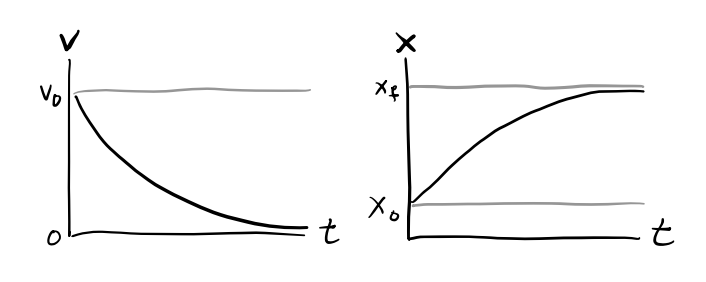
\includegraphics[width=5.20833in,height=\textheight]{classical-mechanics/./resources/image-20230214033729125.png}

}

\end{figure}

Linear drag is frequently used to model objects moving through a viscous
medium at low speeds. Suppose a spherical object of radius \(R\) is
moving slowly in a viscous medium with viscosity \(\eta\). Then the drag
force on the object is given by \textbf{Stokes' Law},

\[
\mathbf{F}_d = -6\pi\eta R \mathbf{v}.
\] This force is linear in velocity, hence we can write
\(F_d = -6\pi\eta R v\), which says the drag constant \(b\) is just

\[
b = 6\pi\eta R.
\]

\hypertarget{example-dropping-a-ball-in-syrup}{%
\subsection{Example: Dropping a ball in
syrup}\label{example-dropping-a-ball-in-syrup}}

Suppose a ball of radius \(R\) and mass \(m\) is dropped in a viscous
syrup from rest at \(x=0\). Find the velocity and position of the ball
as it moves through the fluid.

\begin{figure}

{\centering 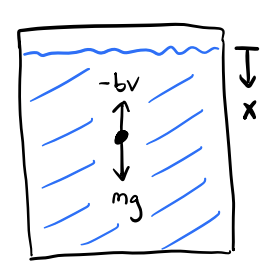
\includegraphics[width=1.5625in,height=\textheight]{classical-mechanics/./resources/image-20230214034514241.png}

}

\end{figure}

This is a 1-dimensional motion problem since the ball is dropped from
rest under gravity, with \(F=F_d + mg\). Here Stoke's law applies, so
the drag force is \(F_d = -bv = -b\dot x\). Plugging into Newton's
Second Law, we have \[
m\ddot x + b \dot x = g.
\] Re-writing this in terms of \(v = \dot x\), we get \[
m \dot v + bv = g,
\] which is a first order linear differential equation for the velocity
\(v(t)\). Its general solution is given by \[
v(t) = v_0 e^{-\frac{b}{m}t} + \frac{mg}{b}(1-e^{-\frac{b}{m}t}).
\] Notice that as \(t \rightarrow \infty\),
\(v(t) \rightarrow \frac{mg}{b}\). That is, \(v(t)\) tends toward a
\textbf{terminal velocity} \[
v_t = \frac{mg}{b} = \frac{mg}{6\pi\eta R}.
\] Since the ball is dropped from rest, \(v_0=0\). The velocity of the
ball is thus given by \[
v(t) = v_t(1-e^{-\frac{b}{m}t}).
\] Using this we can solve for the position to get \[
x(t) = v_t\bigg(t - \frac{b}{m}(1 - e^{-\frac{b}{m}t})\bigg).
\] Notice that drag causes the ball to fall much slower than it would in
free-fall. Instead of being a quadratic function of time, \(x(t)\) is
now approximately a linear function of time, with \(x(t) \sim v_t t\)
for large \(t\).

\begin{figure}

{\centering 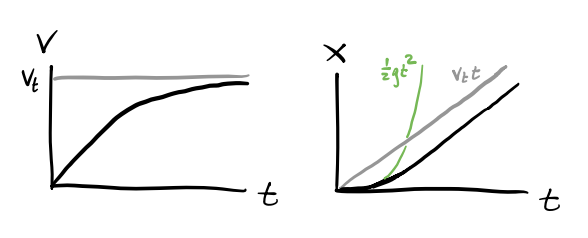
\includegraphics[width=4.16667in,height=\textheight]{classical-mechanics/./resources/image-20230214043325681.png}

}

\end{figure}

\hypertarget{quadratic-drag}{%
\subsection{Quadratic Drag}\label{quadratic-drag}}

We'll now look at quadratic drag, where \(b=0\). Then we get the
differential equation, \[
m\ddot x + c \dot x^2 = 0.
\] This is no longer a linear differential equation due to the
appearance of \(\dot x^2\), but surprisingly we can still solve it using
separation of variables. Again, let \(v = \dot x\). Then we get \[
m\dot v + cv^2 = 0.
\] Rearranging and solving for \(v(t)\), we have \[
\frac{dv}{dt} = -\frac{c}{m}v^2 \quad \Longrightarrow \quad
\int_{v_0}^{v} \frac{dv}{v^2} = -\frac{c}{m} t \quad \Longrightarrow \quad
v(t) = \frac{1}{\frac{1}{v_0} + \frac{c}{m}t}.
\] Integrating both sides and solving for the position, we get \[
x(t) = x_0 + \int_0^t \frac{dt}{\frac{1}{v_0} + \frac{c}{m}t} = x_0 + \frac{m}{c}\log\bigg( 1 + \frac{cv_0}{m}t \bigg).
\] In this case, \(v \rightarrow 0\), but \(x \rightarrow \infty\) as
\(t \rightarrow \infty\). Evidently, while linear drag is strong enough
to slow a moving particle back down to rest, quadratic drag is not.

\begin{figure}

{\centering 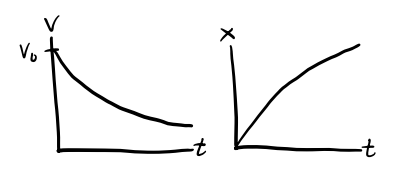
\includegraphics[width=4.16667in,height=\textheight]{classical-mechanics/./resources/image-20230214045706509.png}

}

\end{figure}

Quadratic drag is often used to model the drag experienced by objects
moving through air or other media where pressure is more important than
viscosity. For an object moving through air, drag is well-modeled by the
\textbf{drag equation}, \[
\mathbf{F}_d = -\frac{1}{2}C \rho A v^2 \mathbf{e}_v,
\] where \(\rho\) is the density of air, \(A\) is the cross-sectional
area of the object in the direction of motion, and \(C\) is the
\emph{drag coefficient}. Since this force is proportional to \(v^2\), we
evidently have \[
c = \frac{1}{2}C \rho A.
\]

\hypertarget{reynolds-number}{%
\subsection{Reynold's Number}\label{reynolds-number}}

In practice, how can we tell if drag is in the linear or quadratic
situation? A simple way to do this is by looking at the \emph{Reynold's
Number}. Let's go back to the full quadratic equation for drag, with
\(a\) set to \(0\), \[
F_d = -bv - cv^2.
\] Notice that the ratio \(\frac{cv}{b}\) gives the relative importance
of the two drag terms. Using Stoke's Law and the Drag Equation for the
drag constants, we can re-write this expression as \[
\frac{cv}{b} = \frac{\frac{1}{2}C \rho Av}{6\pi\eta R} = \frac{C \rho Rv}{3\eta}.
\] This ratio is usually rescaled by a factor of \(\frac{3}{C}\) to get
the \textbf{Reynold's number} \(r\), \[
r = \frac{\rho Rv}{\eta}.
\] The Reynold's number is usually what's used in practice to decide
whether we're in the linear or quadratic drag regime.

\begin{itemize}
\tightlist
\item
  When the Reynold's number is \emph{low}, \(r \ll 1\),
  \(v \ll \frac{\eta}{R\rho}\), and we're in the linear regime.
\item
  When the Reynold's number is \emph{high}, \(r \gg 1\),
  \(v \gg \frac{\eta}{R\rho}\), and we're in the quadratic regime.
\item
  The edge case is when \(r \approx 1\), or
  \(v \approx \frac{\eta}{R\rho}\). Then, we have to include \emph{both}
  the linear and quadratic drag terms in the equation of motion. In this
  general case, there's no analytic solution and we have to solve things
  numerically.
\end{itemize}

The Reynold's number is usually easy to calculate since we can often at
least roughly estimate the object's velocity and radius, and we can
usually look up the medium's viscosity and density. For example, a
baseball thrown in air at 100 mph would have a Reynold's number of about
\(r \approx 3 \cdot 10^5 \gg 1\), which is solidly in the quadratic drag
regime.

\hypertarget{harmonic-oscillation}{%
\section{Harmonic Oscillation}\label{harmonic-oscillation}}

The next case we'll consider is when the force is linear in position, \[
\mathbf{F} = -k \mathbf{x}.
\] This relationship is called \textbf{Hooke's Law}. In the
1-dimensional case, it reduces to the equation of motion \[
m \ddot x + kx = 0.
\] This is a second-order linear differential equation for \(x(t)\). The
general solution to this differential equation depends on the sign of
\(k\). If \(k < 0\), we have \[
x(t) = c_1 e^{\frac{k}{m}t} + c_2 e^{-\frac{k}{m}t}.
\] Since \(x \rightarrow \infty\) pretty quickly as
\(t \rightarrow \infty\), this kind of solution is usually non-physical,
except perhaps in situations where \(x\) is bounded between some known
range.

The most important case by far is when \(k > 0\). In this setting, it's
typical to define \(\omega^2 \equiv \frac{k}{m}\) and re-rewrite the
equation as \[
\ddot x + \omega^2 x = 0.
\] This is called the \textbf{simple harmonic oscillator} or
\textbf{SHO}. The canonical example of SHO is of course the motion of a
mass attached to an ideal spring with spring constant \(k\).

The general solution to SHO is a linear combination of sine and cosine
functions, \[
x(t) = c_1 \cos \omega t + c_2 \sin \omega t.
\] This trajectory is oscillatory and stable since it only involves
sines and cosines, both of which are bounded periodic functions. It's
custom to re-write this equation in a more useful form using trig
identities,

\begin{figure}

{\centering 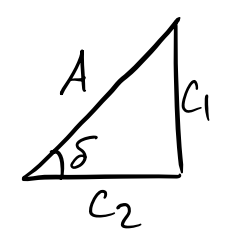
\includegraphics[width=1.5625in,height=\textheight]{classical-mechanics/./resources/image-20230214055348215.png}

}

\end{figure}

\[
\begin{align*}
x(t) &= c_1 \cos \omega t + c_2 \sin \omega t \\
&= A\bigg(\frac{c_1}{A}\cos \omega t + \frac{c_2}{A}\sin\omega t \bigg) \\
&= A(\cos\delta \cos \omega t + \sin\delta\sin\omega t) \\
&= A\cos(\omega t - \delta). \\
\end{align*}
\] In this form, \(A\) is the \textbf{amplitude} of oscillation and
\(\delta\) is the \textbf{phase} of oscillation. The period of
oscillation is given by \[
\tau = \frac{2\pi}{\omega} = 2\pi\sqrt{\frac{m}{k}}.
\]

\begin{figure}

{\centering 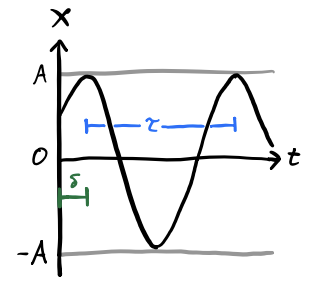
\includegraphics[width=3.125in,height=\textheight]{classical-mechanics/./resources/image-20230214060424511.png}

}

\end{figure}

It's usually convenient when dealing with harmonic oscillators to work
in the complex plane. Consider the complex form of SHO, given by the
differential equation \[
\ddot z + \omega^2 z = 0,
\] where \(z = x+iy = |z|e^{i\theta}\) is a complex variable. Its
general solution is given as a linear combination of complex
exponentials, \[
z(t) = \tilde c_1 e^{i\omega t} + \tilde c_2 e^{-i\omega t}.
\] If we demand that the real solution we seek be given by
\(x(t) = \text{Re}(z(t))\), then

\[
\begin{align*}
x(t) &= \Re(c_1 e^{i \omega t}) + \Re(c_2 e^{-i \omega t}) \\
&= \frac{1}{2}(c_1 + c_2^*)e^{i \omega t} + \frac{1}{2}(c_1^* + c_2)e^{-i \omega t} \\
&= \frac{1}{2} C e^{i \omega t} + \frac{1}{2} C^* e^{-i \omega t} \\
&= A \cdot \Re(e^{i(\omega t - \delta)}) \\
&= A \cos(\omega t - \delta),
\end{align*}
\] where \(C \equiv Ae^{i \delta}\) is some complex number whose real
and imaginary parts are \(c_1+c_2^*\) and \(c_1^*+c_2\) respectively.
For the full complex solution we can similarly write \[
z(t) = A e^{i(\omega t - \delta)}
\] Evidently then, SHO is just a CCW circular rotation in the complex
plane with radius \(A\).

\begin{figure}

{\centering 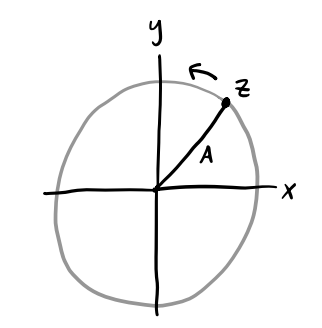
\includegraphics[width=2.08333in,height=\textheight]{classical-mechanics/./resources/image-20230215084009899.png}

}

\end{figure}

\hypertarget{example-bottle-sloshing-in-a-bucket}{%
\subsection{Example: Bottle sloshing in a
bucket}\label{example-bottle-sloshing-in-a-bucket}}

Suppose a bottle of mass \(m\) floats calmly in a bucket of water of
density \(\rho\) at some equilibrium depth of \(d=d_0\). Suppose we push
down slightly on the bottle, perturbing its depth to \(d = d_0 + x\).
The bottle will begin to oscillate. Find its period of oscillation
\(\tau\).

\begin{figure}

{\centering 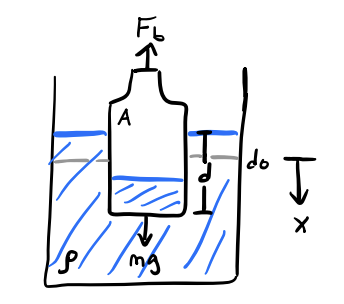
\includegraphics[width=2.08333in,height=\textheight]{classical-mechanics/./resources/image-20230215084145892.png}

}

\end{figure}

The forces on the bottle are gravity downward and an opposing buoyant
force upward, \[
F = mg - \rho g V_{sub} = mg - \rho g A(d_0 + x).
\] At equilibrium, the forces must balance, so
\(0 = mg - \rho g A d_0\), which means \(d_0 = \frac{m}{\rho A}\) is the
equilibrium depth. Simplifying, this says the equation of motion is
given by \[
m \ddot x = mg - \rho g A(d_0 + x) = -\rho g A x = -\frac{mg}{d_0} x.
\] This is just SHO with spring constant \(k = \frac{mg}{d_0}\), or
angular frequency \(\omega = \frac{g}{d}\). Thus, the period of the
bottle's oscillation when \(x\) is small is given by \[
\tau = \frac{2 \pi}{\omega} = 2\pi\sqrt{\frac{d_0}{g}}.
\]

\hypertarget{two-dimensional-harmonic-oscillation}{%
\subsection{Two-Dimensional Harmonic
Oscillation}\label{two-dimensional-harmonic-oscillation}}

Suppose now we allow a mass to move in two dimensions. Hooke's Law
becomes

\[
\begin{align*}
m \ddot x &= -k_x x, \\
m \ddot y &= -k_y y.
\end{align*}
\] Since the equation of motions are uncoupled, the solutions are simply
given by

\[
\begin{align*}
x(t) &= A_x \cos(\omega_x t - \delta_x), \\
y(t) &= A_y \cos(\omega_y t - \delta_y).
\end{align*}
\] Despite what intuition might suggest, the motion of the mass is now
quite non-trivial. In fact, the behavior of the trajectory depends
entirely on the ratio of the frequencies \(\frac{\omega_x}{\omega_y}\)
and the relative phase between the two oscillations
\(\delta = \delta_x - \delta_y\).

The motion will only be periodic if \(\frac{\omega_x}{\omega_y}\) is
\emph{rational}, i.e.~if the frequencies are integer multiples of each
other. The curves traced out by \((x(t), y(t))\) when
\(\frac{\omega_x}{\omega_y}\) is rational are called \textbf{Lissajous
curves}. They can get quite complicated, but they'll always be periodic.
Here's what a few of them look like for
different\(\frac{\omega_x}{\omega_y}\) and \(\delta\).

\begin{figure}

{\centering \includegraphics[width=4.16667in,height=\textheight]{https://upload.wikimedia.org/wikipedia/commons/4/47/Lissajous_relaciones.png}

}

\end{figure}

\hypertarget{example-charged-particle-in-a-uniform-magnetic-field}{%
\subsection{Example: Charged particle in a uniform magnetic
field}\label{example-charged-particle-in-a-uniform-magnetic-field}}

Suppose a particle with charge \(q\) and mass \(m\) is moving in the
presence of a constant magnetic field \(\mathbf{B}\). Find its equations
of motion, solve for the trajectory, and describe what it looks like.

\begin{figure}

{\centering 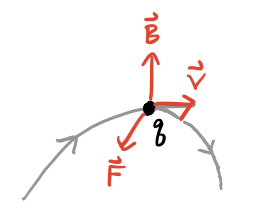
\includegraphics[width=2.08333in,height=\textheight]{classical-mechanics/./resources/image-20230215094609106.png}

}

\end{figure}

If \(\mathbf{v}\) is the velocity of the particle, the magnetic force is
given by \(\mathbf{F} = \frac{q}{c} \mathbf{v} \times \mathbf{B}\).
Suppose \(\mathbf{B} = B \mathbf{e}_z\). Then \[
\mathbf{F} = \frac{q}{c}\mathbf{v} \times \mathbf{B} = \frac{qB}{c}(\dot y \mathbf{e}_x - \dot x \mathbf{e}_y),
\] The equations of motion are thus

\[
\begin{align*}
m \ddot x &= \frac{qB}{c} \dot y , \\
m \ddot y &= -\frac{qB}{c} \dot x , \\
m \ddot z &=  0. \\
\end{align*}
\] Define \(\omega \equiv \frac{qB}{c}\). The first two equations can be
decoupled to give two independent SHO equations in the velocities,

\[
\begin{align*}
\ddot v_x &= -\omega^2 v_x , \\
\ddot v_y &= -\omega^2 v_y , \\
\end{align*}
\] with solutions

\[
\begin{align*}
v_x(t) &= V_x \cos(\omega t - \delta_x) , \\
v_y(t) &= V_y \cos(\omega t - \delta_y)  , \\
\end{align*}
\] Now, since \(\ddot v_x = \omega \dot v_y\), we must have
\(V_x = V_y\) and \(\delta_y = \delta_x - \frac{\pi}{2}\). Taking
\(\delta_x=0\) and \(V_x = R\omega\) for convenience, we get

\[
\begin{align*}
v_x(t) &= R\omega \cos(\omega t) , \\
v_y(t) &= -R\omega \sin(\omega t)  , \\
\end{align*}
\] Finally, integrating the velocity equations gives the trajectory,

\[
\begin{align*}
x(t) &=  x_0 + R \sin(\omega t), \\
y(t) &= (y_0 - R) + R \cos(\omega t) , \\
z(t) &=  z_0 + v_{0z} t. \\
\end{align*}
\] This is just a helix of radius \(R\) directed along the z-axis. That
is, the particle will just spiral around in a helix directed along the
line of the magnetic field. The frequency \(\omega\) is called the
\emph{cyclotron frequency}. Since charge can be positive or negative, it
carries a sign, which determines which way the particle will spiral.
Notice that \(R\) is just the radius of orbit. It's customarily
expressed in terms of the tangential velocity
\(v_\perp = \sqrt{v_x^2 + v_y^2} = R\omega\), \[
R = \frac{mcv_\perp}{qB}.
\]

\begin{figure}

{\centering 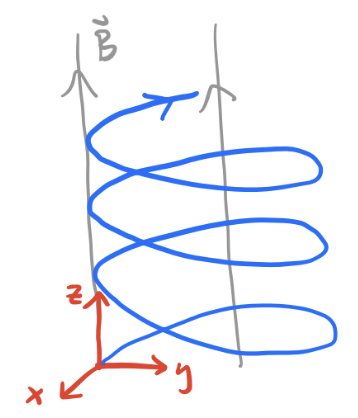
\includegraphics[width=2.08333in,height=\textheight]{classical-mechanics/./resources/image-20230215095809160.png}

}

\end{figure}

\hypertarget{damped-harmonic-oscillation}{%
\section{Damped Harmonic
Oscillation}\label{damped-harmonic-oscillation}}

Let's now combine the forces of linear drag with the forces of harmonic
oscillation. In the 1-dimensional case, this gives the \textbf{damped
harmonic oscillator} or \textbf{DHO}, \[
m \ddot x + bx + kx = 0.
\] Define \(\beta \equiv \frac{b}{2m}\) and
\(\omega_0 \equiv \sqrt{\frac{k}{m}}\), called the \textbf{damping
constant} and the \textbf{natural frequency} respectively. Then we can
write the DHO equation of motion as \[
\ddot x + 2\beta x + \omega_0^2 x = 0.
\] It'll be insightful to solve this in its complex form. Consider
instead the equation \[
\ddot z + 2\beta z + \omega_0^2 z = 0,
\] where \(z\) is complex-valued. Let's try and assume a trial solution
of the form \(z = A e^{i\omega t - \delta}\). Plugging this into the
differential equation, we get \[
(-\omega^2 + 2\beta + \omega_0^2)A e^{i\omega t - \delta} = 0.
\] In the non-trivial case \(A \neq 0\), this implies
\((-\omega^2 + 2\beta + \omega_0^2) = 0\), which we can solve for
\(\omega\) to get \[
\omega = i\beta \pm \sqrt{\omega_0^2 - \beta^2} \equiv i\beta \pm \omega',
\] where \(\omega' \equiv \sqrt{\omega_0^2 - \beta^2}\). Plugging this
into \(z\) then gives \[
z(t) = e^{-\beta t}(c_1 e^{i\omega' t} + c_2 e^{-i\omega' t}).
\] When dealing with damped systems, it's customary to define a
\textbf{quality factor} \(Q \equiv \frac{\omega_0}{2\beta}\), which
expresses in relative terms how much the system is being damped. We can
re-write \(\omega'\) in terms of the Q-factor as \[
\omega' = \omega_0 \sqrt{1 - \bigg(\frac{1}{2Q}\bigg)^2}.
\] Evidently, the form of the solutions divide into three cases
depending on the sign of \(\omega'\):

\begin{enumerate}
\def\labelenumi{\arabic{enumi}.}
\item
  Underdamping (\(\omega' > 0\) or \(Q < \frac{1}{2}\)): In this case,
  \(\omega'\) is real, which means we have a real solution \[
  x(t) = A e^{-\beta t} \cos(\omega't - \delta).
  \] This is an exponentially damped sinusoidal oscillation, where
  \(x \rightarrow 0\) with time constant \(\tau = \frac{1}{\beta}\).
  Notice \(\omega' < \omega_0\), which means the \emph{actual} frequency
  of the oscillation is \emph{less} than the natural frequency. When
  \(Q \gg 1\) this distinction disappears, since
  \(\omega' \approx \omega_0\). In practice this occurs frequently for
  underdamped solutions, and \(Q\) need not even be large for
  \(\omega' \approx \omega_0\).

  \begin{figure}

  {\centering 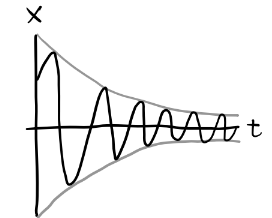
\includegraphics[width=2.08333in,height=\textheight]{classical-mechanics/./resources/image-20230215123127416.png}

  }

  \end{figure}
\item
  Overdamping (\(\omega' < 0\) or \(Q > \frac{1}{2}\)): In this case,
  \(\omega'\) is complex. Define \(\kappa \equiv i\omega'\), which is
  real-valued. Then we have a solution of the form \[
  x(t) = e^{-\beta t}(c_1 e^{\kappa t} + c_2 e^{-\kappa t}).
  \] Since \(\kappa < \beta\), \(x \rightarrow 0\) monotonically, with
  time constant \(\tau = \frac{1}{\beta - \kappa}\).

  \begin{figure}

  {\centering 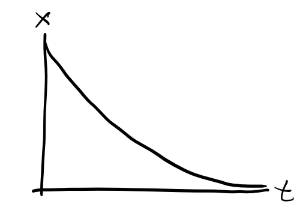
\includegraphics[width=2.08333in,height=\textheight]{classical-mechanics/./resources/image-20230215123205612.png}

  }

  \end{figure}
\item
  Critical damping (\(\omega' = 0\) or \(Q = \frac{1}{2}\)): This is the
  edge case where \(\omega_0 = \beta\) exactly. Here the solution is
  degenerate, with \[
  x(t) = (c_1 + c_2 t) e^{-\beta t}.
  \] Again, \(x \rightarrow 0\), but with time constant
  \(\tau = \frac{1}{\beta}\). Evidently, the critically damped solution
  decays faster than the overdamped solution.

  \begin{figure}

  {\centering 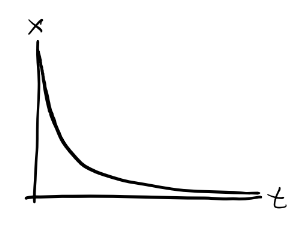
\includegraphics[width=2.08333in,height=\textheight]{classical-mechanics/./resources/image-20230215123225987.png}

  }

  \end{figure}
\end{enumerate}

In all three cases the system must \emph{eventually} come to rest due to
the presence of damping. Only the ``high Q'' systems are allowed to
oscillate. Note that as \(\beta \rightarrow 0\),
\(Q \rightarrow \infty\). In this limit the solution turns into regular
SHO, with \(\omega' \rightarrow \omega_0\).

\hypertarget{driven-damped-harmonic-oscillation}{%
\section{Driven Damped Harmonic
Oscillation}\label{driven-damped-harmonic-oscillation}}

Let's now add in the independent force term to the mix. In the
1-dimensional case, we get the equation of motion \[
m \ddot x + b \dot x + kx = F_0(t).
\] This is called the \textbf{driven damped harmonic oscillator} or
\textbf{DDHO}. We imagine \(F_0(t)\) to be some external \textbf{driving
force} acting on the system. It's again convenient to rewrite things by
defining \(\beta = \frac{b}{2m}\), \(\omega_0^2 = \frac{k}{m}\), and
\(f(t) = \frac{F_0(t)}{m}\). Then we have the linear differential
equation \[
\ddot x + 2\beta\dot x + \omega_0^2 x = f(t).
\] Recall that the solutions of linear differential equations can be
decomposed into two pieces, a \emph{homogenous solution} and a
\emph{particular solution}. The homogenous solution is the general
solution to \[
\ddot x_h + 2\beta\dot x_h + \omega_0^2 x_h = 0.
\] But this is just a DHO. We solved that part already. All we need to
do now is find any particular solution that will solve \[
\ddot x_p + 2\beta\dot x_p + \omega_0^2 x_p = f(t).
\] Provided we do that, the full, general solution will be
\(x(t) = x_h(t) + x_p(t)\). There are several ways to find a particular
solution, including guessing methods and more systematic methods like
Green functions and Fourier transforms. We'll briefly touch on some of
these.

\hypertarget{example-underdamped-hanging-spring}{%
\subsection{Example: Underdamped hanging
spring}\label{example-underdamped-hanging-spring}}

Suppose a spring is suspended vertically from a ceiling under the
presence of gravity. Find the position \(x=x(t)\). Also, find the amount
that gravity changes the spring's equilibrium length.

\begin{figure}

{\centering 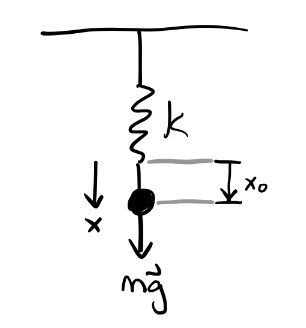
\includegraphics[width=2.08333in,height=\textheight]{classical-mechanics/./resources/image-20230215134622171.png}

}

\end{figure}

The forces in this problem are gravity, linear drag, and a spring force,
so if \(x\) points downward, \[
F = mg - bv - kx.
\] The equation of motion is thus given by \[
m \ddot x + b \dot x + kx = mg.
\] This is just DDHO with \(f(t) = g\). We thus seek a particular
solution \(x_p(t)\) such that \[
\ddot x_p + 2\beta\dot x_p + \omega_0^2 x_p = g.
\] Assume a trial solution of the form \(x_p = c\). Then, \[
\omega_0^2 c = g \Longrightarrow c = \frac{g}{\omega_0^2} = \frac{gm}{k}.
\] Supposing the spring is underdamped, then \[
x(t) = Ae^{-\beta t} \cos(\omega' t - \delta) + \frac{gm}{k}.
\] The new equilibrium occurs when the object is at rest, i.e.~when
\(\ddot x = \dot x = 0\). This occurs at \(x = \frac{gm}{k}\) relative
to the free equilibrium \(x=0\).

\hypertarget{sinusoidal-driving-forces}{%
\subsection{Sinusoidal Driving Forces}\label{sinusoidal-driving-forces}}

The most interesting driving forces in practice are ones that are
periodic. Periodic driving functions lead to the important concept of
\textbf{resonance}, which is a phenomenon that occurs when the driving
frequency matches the natural frequency.

Consider a sinusoidal driving force of the form
\(f(t) = f_0 \cos\omega t\). In complex form, we can then write \[
\ddot z + 2\beta\dot z + \omega_0^2 z = f_0 e^{i \omega t}.
\] Assume a particular solution of the form
\(z(t) = \tilde A e^{i \omega t}\) where \(\tilde A = Ae^{-i\delta}\).
Plugging this in, we have \[
(-\omega^2 + 2\beta\omega i + \omega_0^2)\tilde A e^{-i\omega t} = f_0 e^{i\omega t},
\] which we can solve for the complex amplitude \(\tilde A\) to get \[
\tilde A = \frac{f_0}{(\omega_0^2-\omega^2) + 2\beta\omega i}.
\] With the help of little trig, we can decompose this solution to get
the real amplitude and phase,

\begin{figure}

{\centering 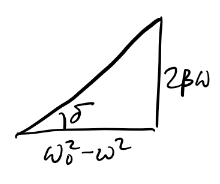
\includegraphics[width=1.5625in,height=\textheight]{classical-mechanics/./resources/image-20230215141606559.png}

}

\end{figure}

\[
A = \frac{f_0}{\sqrt{(\omega_0^2-\omega^2)^2 + 4\beta^2\omega^2}}, \quad \delta = \tan^{-1} \frac{2\beta\omega}{\omega_0^2-\omega^2}.
\]

With these, the real particular solution is given by
\(x_p(t) = A \cos(\omega t - \delta)\). Since the homogenous solution
decays to zero exponentially, \(x \rightarrow x_p\) as
\(t \rightarrow \infty\). That is, \(x_p(t)\) describes the \emph{steady
state solution} of the DDHO. In this sense, the system evidently
``forgets'' its own natural frequency and starts to oscillate at the
driving frequency as time goes on and the transient state dies off.

\begin{figure}

{\centering 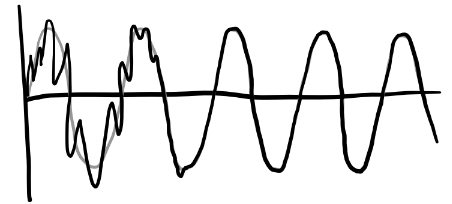
\includegraphics[width=3.125in,height=\textheight]{classical-mechanics/./resources/image-20230215142723690.png}

}

\end{figure}

Interestingly, the memory of the transient dynamics \emph{is} preserved
in the amplitude and phase. As a rule of thumb, the number of
oscillations \(N\) until \(x \approx x_p\) is basically just the
Q-factor, \[
N \approx \frac{Q}{\pi}.
\] Let's now look more deeply at the amplitude and phase. It's worth
asking how they depend on the external driving frequency \(\omega\).

\begin{itemize}
\tightlist
\item
  When \(\omega \ll \omega_0\), \(A \approx \frac{f_0}{\omega_0^2}\) and
  \(\delta \approx 0\).
\item
  When \(\omega \gg \omega_0\), \(A \approx 0\) and
  \(\delta \approx \pi\).
\item
  When \(\omega \approx \omega_0\),
  \(A \approx \frac{f_0}{2\beta\omega_0}\) and
  \(\delta \approx \frac{\pi}{2}\).
\end{itemize}

\begin{figure}

{\centering 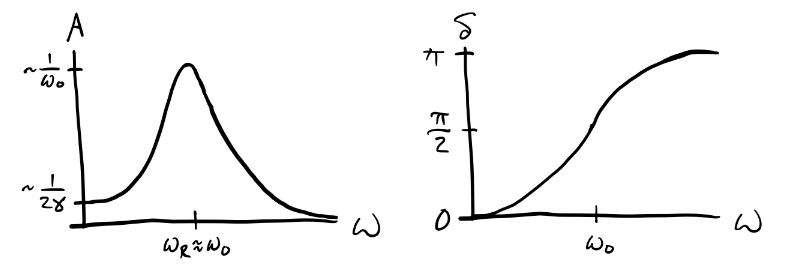
\includegraphics[width=5.20833in,height=\textheight]{classical-mechanics/./resources/image-20230215145247903.png}

}

\end{figure}

Evidently, \(A\) is maximized at
\(\omega_R = \sqrt{\omega_0^2-2\beta^2} = \omega_0 \sqrt{1-\frac{1}{2Q^2}}\).
When \(Q>1\), \(\omega_R \approx \omega_0\), so this distinction doesn't
really matter. This frequency \(\omega_R \approx \omega_0\) is called
the \textbf{resonance frequency} of the system. When the driver is
operating near the resonance frequency, the system responds extremely
well to the driving force. It turns out that when a spectrum of
frequencies is dumped on an oscillating system, the system tends to pick
out the resonance frequencies and respond to those. This fact makes
resonance a very important topic in physics and engineering.

In practice, high-Q systems are very common. In those cases, \(A\) dies
off quickly when the driving frequencies aren't close to \(\omega_0\).
That means practically all the interesting behavior of a high-Q systems
is in the band around the resonance frequency. Suppose
\(\Delta \equiv \omega - \omega_0\) is small. Then we can write \[
(\omega_0^2-\omega^2) = (\omega_0-\omega)(\omega_0+\omega) = -\Delta(2\omega_0+\Delta) \approx -2\omega_0 \Delta.
\] That means we can write the complex amplitude \(\tilde A\) as \[
\tilde A = \frac{f_0}{(\omega_0^2-\omega^2) + 2\beta\omega i} \approx -\frac{\frac{f_0}{2\omega_0}}{\Delta-\beta i} = \frac{f_0}{2\omega_0}\bigg(-\frac{\Delta}{\Delta^2+\beta^2} + i\frac{\beta}{\Delta^2+\beta^2} \bigg).
\] This function on the right is called the \textbf{Lorentzian}. Using
this, we can see \[
A \approx \frac{f_0}{2\omega_0} \frac{1}{\sqrt{\Delta^2 + \beta^2}} \quad \Longrightarrow \quad A^2 \approx \bigg(\frac{f_0}{2\omega_0}\bigg)^2 \frac{1}{\Delta^2 + \beta^2}.
\] Since the energy in a harmonic oscillator is just
\(E = \frac{1}{2}kA^2 \propto A^2\), it's common to look at plots of
\(A^2\) when plotting these \textbf{resonance curves}. Evidently,
\(A^2 \rightarrow 0\) as \(\Delta \rightarrow \infty\), and it's
maximized when \(\Delta = 0\), which is when \(\omega = \omega_0\) and
\(A_{max}^2 = \big(\frac{f_0}{2\omega_0 \beta}\big)^2\).

It's common to measure the \emph{width} of the resonance curve by using
the \textbf{full width at half maximum} or \textbf{FWHM}. The FWHM is
defined as the difference between the left and right points around the
maximum whose height is half the maximum, \[
FWHM \equiv \Delta \omega \equiv \omega_R - \omega_L, \quad \text{where} \quad A^2(\omega_L) = A^2(\omega_R) = \frac{1}{2}A_{max}.
\] Solving for these left and right points gives
\(\omega_L = \omega_0 - \beta\) and \(\omega_R = \omega_0 + \beta\), so
\[
\Delta \omega = (\omega_0 + \beta) - (\omega_0 - \beta) = 2\beta.
\] The \emph{resolving power} of the resonance curve is then \[
\frac{\omega_0}{\Delta} = \frac{\omega_0}{2\beta} = Q.
\] Evidently then, \(Q\) represents the resolving power of the resonance
curve. The higher the Q-factor is, the more sharply peaked the resonance
curve is, and the easier we can pinpoint the resonance frequency
exactly. Indeed, this is why \(Q\) is called a \emph{quality factor}.

\begin{figure}

{\centering 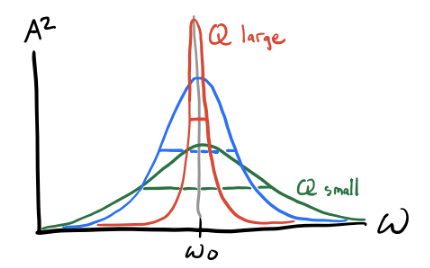
\includegraphics[width=3.125in,height=\textheight]{classical-mechanics/./resources/image-20230215154645401.png}

}

\end{figure}

One very important system where we want a high-Q is a \emph{clock}. To
keep precise time, we need to make sure that it's oscillating pretty
much \emph{exactly} at its resonance frequencies. This is because we
need to keep a regular period, so \(\tau = \frac{2\pi}{\omega}\) can't
be allowed to vary very much from the true period
\(\tau_0 = \frac{2\pi}{\omega_0}\). There's a tradeoff though. Since the
decay time of the transient behavior is
\(N\tau_0 \equiv \frac{1}{\beta}\), it takes about \(N=\frac{Q}{\pi}\)
cycles of \emph{ringing} for the system to come to steady state. So the
better precision we want, the longer we'll have to wait for the system
to come to steady state.

Note that \(Q\) also affects the \emph{phase curve} of the system, since
\[
\delta = \tan^{-1} \frac{2\beta\omega}{\omega_0^2-\omega^2} \approx \tan^{-1} \frac{2\omega}{Q\Delta}.
\] Evidently as \(Q\) increases, the system becomes more responsive to
sudden changes in phase around \(\omega_0\).

\begin{figure}

{\centering 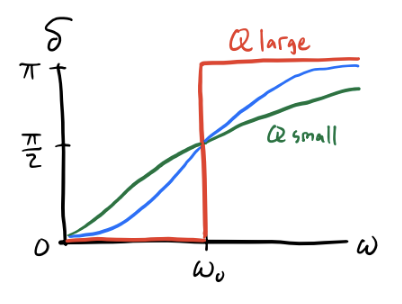
\includegraphics[width=3.125in,height=\textheight]{classical-mechanics/./resources/image-20230215160032343.png}

}

\end{figure}

\hypertarget{arbitrary-driving-forces}{%
\subsection{Arbitrary Driving Forces}\label{arbitrary-driving-forces}}

The situation where resonance occurs in a DDHO system is not just
confined to sinusoidal driving forces. Using Fourier analysis, we can
decompose more arbitrary driving forces into a sum of sinusoidal driving
forces of different frequencies. The simplest of these cases is when the
driving force is periodic with some period \(\tau\). Even if the driver
isn't sinusoidal, we can decompose it into a linear combination of
cosines of different frequencies, i.e.~a \emph{Fourier Series}, \[
f(t) = \sum_{n=-\infty}^{\infty} f_n e^{i \omega n t},
\] where each \(f_n\) can be found via the formula \[
f_n = \langle f(t), e^{i \omega n t} \rangle = \frac{\omega}{\pi} \int_0^{\tau} f(t) e^{i \omega n t} dt.
\] Using the principle of superposition, we could then find the solution
for each of the sinusoidal drivers term by term, and then sum them
together to get the full solution. Each term will have amplitude and
phase \[
A_n = \frac{f_n}{\sqrt{(\omega_0^2-\omega^2 n^2)^2 + (2\beta\omega n)^2}}, \quad \delta_n = \tan^{-1} \frac{2\beta\omega n}{\omega_0^2-\omega^2n^2}.
\] Plugging these in will yield a general solution of the form \[
x(t) = x_h(t) + \sum_{n=1}^{\infty} A_n \cos(\omega n t - \delta_n).
\] Each component will yield its own resonance frequency where
\(\omega n \approx -\omega_0\). As a function of the main driving
frequency, this means there will resonances at each
\(\omega_n = \frac{\omega_0}{n}\). The resonance curve for \(A^2\) can
be found via \emph{Parseval's Theorem}, which says \[
A^2 = \langle x^2(t) \rangle = \frac{1}{2} \sum_{n=0}^\infty A_n^2.
\] The peaks evidently go to zero as \(n \rightarrow \infty\) since each
\(A_n^2 \propto f_n^2\) and each \(f_n \rightarrow 0\) by the
Riemann--Lebesgue lemma.

\begin{figure}

{\centering 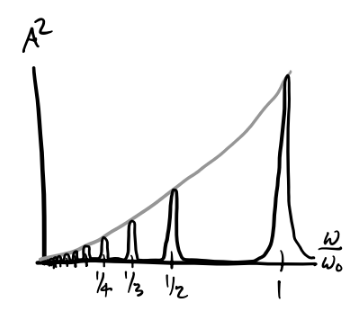
\includegraphics[width=2.60417in,height=\textheight]{classical-mechanics/./resources/image-20230215160201364.png}

}

\end{figure}

What if the driving force isn't periodic? In this case we have a few
options. One would be to decompose it into its \emph{Fourier transform},
\[
f(t) = \int_{-\infty}^{\infty} f(\omega) e^{i\omega t} dt.
\] Then each term gives a set of complex amplitudes and phases that can
be solved for and stitched back together to get \(x(t)\). Another
solution that's perhaps more common is to use \emph{Green's functions}.
Instead of decomposing the driver into a linear combination of periodic
functions, we'll decompose it into a linear combination of \emph{impulse
responses} or \emph{delta functions}, \[
f(t) = \int_{-\infty}^{\infty} f(t') \delta(t-t') dt'.
\] To find the solution \(x(t)\), we first need to find the particular
solution \(G(t-t')\) to the DDHO with an impulse response, \[
\ddot G + 2\beta\dot G + \omega_0^2 G = \delta(t - t').
\] Once this is found, we can stitch together the full solution as \[
x(t) = \int_{-\infty}^{\infty} f(t') G(t-t') dt'.
\] Note the Green's function solution already incorporates in the
homogeneous solution since \(G(t-t')\) must itself satisfy the initial
conditions.

\hypertarget{reference-frames}{%
\chapter{Reference Frames}\label{reference-frames}}

The laws of mechanics as formulated thus far are not valid as written
for every observer. They are valid only for a special class of observers
in \emph{inertial} reference frames. A classical \textbf{inertial
reference frame} is a reference frame or coordinate system in which
Newton's Laws hold with no modifications. That such frames even exist is
an experimental fact of nature.

In practice, however, many reference frames of interest are
\emph{non-inertial}, which means Newton's Laws does not hold in those
reference frames. We have to modify Newton's Laws in these frames by
adding so-called \textbf{fictitious forces}. We'll begin by focusing on
the most common non-inertial frames, the \emph{rotating reference
frames}.

\hypertarget{orthogonal-transformations}{%
\section{Orthogonal Transformations}\label{orthogonal-transformations}}

Suppose \(\mathbf{x}\) is some vector, and \(\{\mathbf{e}_i\}\) and
\(\{\mathbf{e}_i'\}\) are two orthonormal bases for \(\mathbb{R}^3\),
then \[
\mathbf{x} = \sum_{j=1}^3 x_j \mathbf{e}_j = \sum_{i'=1}^3 x_{i'} \mathbf{e}_{i'},
\] where \(x_i = \mathbf{x} \cdot \mathbf{e}_i\) and
\(x_i' = \mathbf{x} \cdot \mathbf{e}_i'\).

\textbf{Notation:} From now on we'll use the \emph{Einstein summation
convention}. If a repeated index occurs in a sum, we'll omit the
\(\sum\) symbol. For example, we can re-write the above line as the
following, where it's understood we're summing over \(j\) and \(i'\) in
each case, \[
\mathbf{x} = x_j \mathbf{e}_j = x_{i'} \mathbf{e}_{i'}.
\] Now, observe we can write one component in terms of the other as \[
x_i' = \mathbf{x} \cdot \mathbf{e}_{i'} = (\mathbf{e}_j \cdot \mathbf{e}_{i'}) x_j \equiv R_{i'j} x_j,
\] where \(R_{i'j} = \mathbf{e}_j \cdot \mathbf{e}_i'\) defines a matrix
\(\mathbf{R}\) called an \textbf{orthogonal transformation}.

Notice that if we take the inner product of two vectors \(\mathbf{x}\)
and \(\mathbf{y}\), we get \[
\mathbf{x} \cdot \mathbf{y} = x_{i'} \delta_{i' j'} x_{j'} = R_{ii'} \delta_{i'j'} R_{j'j} x_i x_j = \mathbf{x} \cdot (\mathbf{R}^\top \mathbf{R}) \mathbf{y}.
\] Thus, an orthogonal transformation \(\mathbf{R}\) satisfies the
property that \[
\mathbf{R}^\top \mathbf{R} = \mathbf{I}, \quad \text{or} \quad R_{ij} R_{jk} = \delta_{ik}.
\] Due to the inner product preserving nature of orthogonal
transformations, they can in a sense be used to \emph{define} what we
mean by a scalar or vector or tensor in classical mechanics. They're
objects that transform a certain way under an orthogonal transformation:

\begin{itemize}
\item
  A \textbf{scalar} is any object \(\alpha\) that is \emph{invariant}
  under an orthogonal transformation, \[
  \alpha' = \alpha.
  \]
\item
  A \textbf{vector} is any object \(\mathbf{v}\) that transforms under
  an orthogonal transformation as, \[
  v_{i'} = R_{i'i} v_i.
  \]
\item
  A \textbf{tensor} of order \(k\) is any object \(\mathbf{T}\) that
  transforms under an orthogonal transformation as, \[
  T_{i_1' i_2' \cdots i_k'} = R_{i_1' i_1} R_{i_2' i_2} \cdots R_{i_k' i_k} T_{i_1 i_2 \cdots i_k}.
  \]
\end{itemize}

Notice since \(\mathbf{R}^\top \mathbf{R} = \mathbf{I}\), we can take
the determinant of both sides to get
\(\det(\mathbf{R}^\top \mathbf{R}) = \det^2(\mathbf{R}) = 1\), which
implies that \(\det(\mathbf{R}) = \pm 1\). This fact divides orthogonal
transformations into two distinct classes:

\begin{itemize}
\tightlist
\item
  Proper Rotations (\(\det(\mathbf{R}) = 1\)): These correspond to pure
  \emph{rotations} in space. They preserve the \emph{handedness} of the
  underlying coordinate system.
\item
  Improper Rotations (\(\det(\mathbf{R}) = -1\)): These correspond to
  \emph{reflections} in space, which are transformations
  \(\mathbf{v} \Rightarrow -\mathbf{v}\) combined with a pure rotation.
  These transformations permute the handedness of the underlying
  coordinate system.
\end{itemize}

\begin{figure}

{\centering 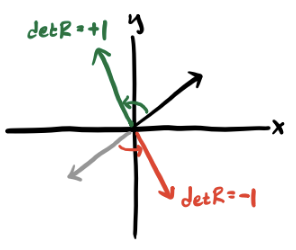
\includegraphics[width=1.875in,height=\textheight]{classical-mechanics/./resources/image-20230216104709404.png}

}

\end{figure}

Most vector operations are proper, in the sense that they preserve the
handedness of the underlying coordinate system. If \(\mathbf{v}\) is a
vector, they'll transform under a reflection to \(-\mathbf{v}\). The one
major exception is the \emph{cross product}, which reverses the
handedness. Under a reflection, it keeps its sign, \[
\mathbf{v} \times \mathbf{w} \Rightarrow (-\mathbf{v}) \times (-\mathbf{w}) = \mathbf{v} \times \mathbf{w}.
\] For this reason, cross products are sometimes called
\textbf{pseudovectors} or \textbf{axial vectors} to distinguish them
from ordinary vectors that transform under a reflection as
\(\mathbf{v} \Rightarrow -\mathbf{v}\).

\textbf{Aside:} It turns out that the set of all orthogonal
transformations on \(\mathbb{R}^3\) form a \emph{group} \(G\), in the
sense that it satisfies the following special ``symmetry'' properties:

\begin{itemize}
\tightlist
\item
  Closure: If \(A, B \in G\) , then \(AB \in G\) also.
\item
  Associativity: For any \(A,B,C \in G\), we have \((AB)C = A(BC)\).
\item
  Identity: There is a unique element \(I \in G\) satisfying \(IA = AI\)
  for any \(A \in G\).
\item
  Invertibility: For any \(A \in G\), there is an inverse element
  \(A^{-1}\) such that \(A^{-1} A = A A^{-1} = I\).
\end{itemize}

The group of orthogonal transformations under matrix multiplication is
called the \textbf{orthogonal group}, denoted \(O(3)\). The subset of
\(O(3)\) where \(\det(\mathbf{R})=1\) happens to form a
\textbf{subgroup}, i.e.~a subset of \(O(3)\) that's closed under group
operations. It's called the \textbf{special orthogonal group}, denoted
\(SO(3)\). This is essentially the group of all rotations in 3
dimensions. The orthogonal groups turn out to be very important in
understanding the theory of angular momentum, especially in quantum
mechanics.

\hypertarget{example-rotations-in-two-dimensions}{%
\subsection{Example: Rotations in two
dimensions}\label{example-rotations-in-two-dimensions}}

We can easily figure out what proper rotations look like in 2D space by
looking at how to relate one basis with another. Suppose
\(\{\mathbf{e}_x, \mathbf{e}_y \}\) is the standard basis for
\(\mathbb{R}^2\), and \(\{\mathbf{e}_{x'}, \mathbf{e}_{y'}\}\) is some
other orthonormal basis. Suppose \(\varphi\) is the angle between
\(\mathbf{e}_x\) and \(\mathbf{e}_{x'}\). Using a little geometry, we
have,

\begin{figure}

{\centering 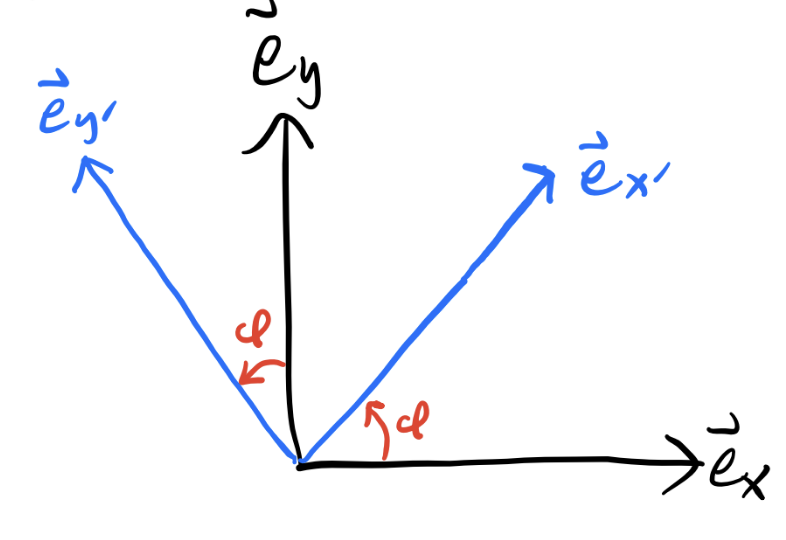
\includegraphics[width=2.08333in,height=\textheight]{classical-mechanics/./resources/image-20230216110516749.png}

}

\end{figure}

\[
\begin{align*}
R_{x'x} &= \mathbf{e}_{x'} \cdot \mathbf{e}_x = \cos\varphi,
&R_{x'y} &= \mathbf{e}_{x'} \cdot \mathbf{e}_y = \sin\varphi, \\
R_{y'x} &= \mathbf{e}_{y'} \cdot \mathbf{e}_x = -\sin\varphi,
&R_{y'y} &= \mathbf{e}_{y'} \cdot \mathbf{e}_y = \cos\varphi. \\
\end{align*}
\] We can thus express any proper rotation in \(\mathbb{R}^2\) using a
\(2 \times 2\) matrix of the form \[
\mathbf{R}(\varphi) = 
\begin{pmatrix}
\cos\varphi & \sin\varphi \\
-\sin\varphi & \cos\varphi
\end{pmatrix}.
\] This is the matrix that rotates the underlying basis
\(\{\mathbf{e}_x, \mathbf{e}_y \}\) to the new, rotated basis
\(\{\mathbf{e}_{x'}, \mathbf{e}_{y'} \}\).

\hypertarget{active-vs-passive-transformations}{%
\subsection{Active vs Passive
Transformations}\label{active-vs-passive-transformations}}

The previous example suggests that we can think about a rotation in
space two different ways. One way is to rotate the underlying basis and
keep the vector \(\mathbf{v}\) fixed. That is,
\(\mathbf{e}_i \Rightarrow R_{i'i} \mathbf{e}_i\).. This way of looking
at a rotation is called a \textbf{passive transformation}. It rotates
the coordinate system under \(\mathbf{v}\), not \(\mathbf{v}\) itself.

Another way of looking at a rotation is to imagine keeping the
coordinate system fixed, but rotating the components of the vector
\(\mathbf{v}\) directly. That is, \(v_i \Rightarrow R_{i'i}v_i\). This
way of looking at a rotation is called an \textbf{active
transformation}. Despite sounding semantically different, these two ways
are physically equivalent. Note though that if a vector rotates actively
under \(\mathbf{R}(-\varphi)\), it will rotate passively under
\(\mathbf{R}(\varphi)\).

\begin{figure}

{\centering 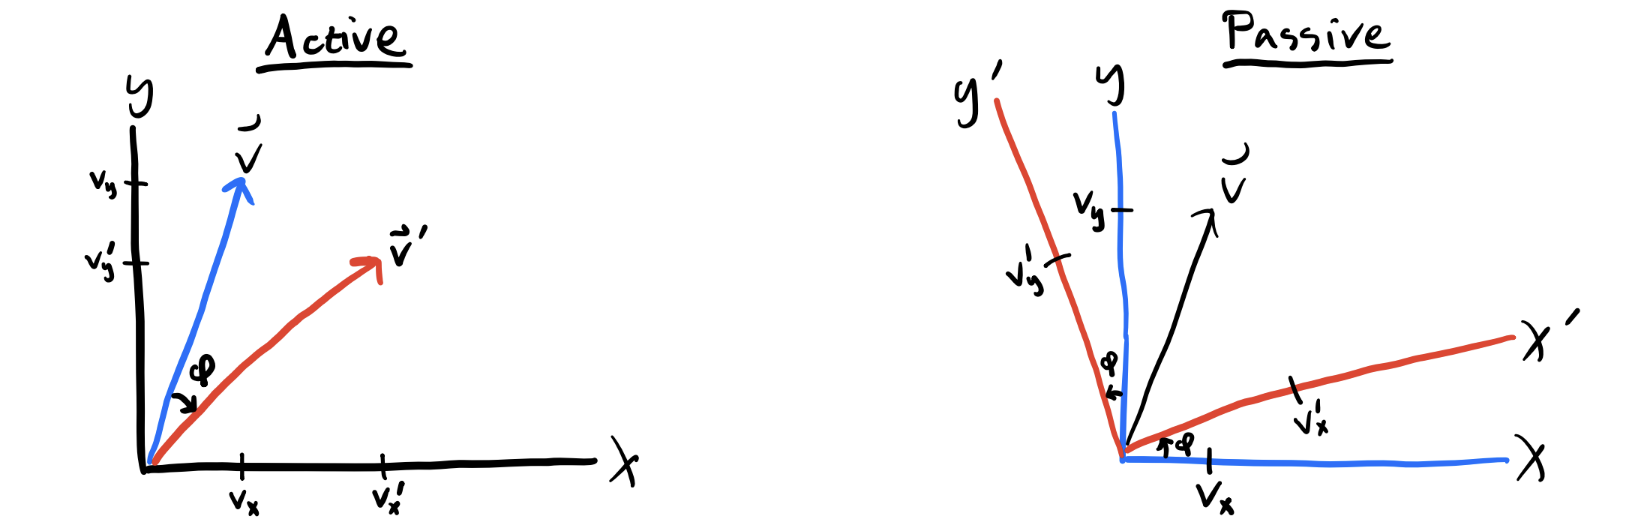
\includegraphics[width=7.29167in,height=\textheight]{classical-mechanics/./resources/image-20230216112859340.png}

}

\end{figure}

It's usually more convenient to assume rotations are active
transformations. The major exception is when dealing with rigid bodies,
where it's more convenient to passively transform to body coordinates.
Note the same logic applies to 3D transformations. In that case, there
are now three angles of rotation to deal with, not just one.

\hypertarget{linearly-accelerating-frames}{%
\section{Linearly Accelerating
Frames}\label{linearly-accelerating-frames}}

Let's now examine the motion of systems in non-inertial reference
frames. In examining accelerating frames, we'll treat them as static
coordinate systems, completely ignoring the forces that \emph{cause} the
reference frame to accelerate in the first place. We'll start with
linearly accelerating frames.

Suppose a system is ``locked into'' a reference frame \(S_{rel}\), which
is itself moving at a velocity \(\mathbf{v}_0\) with respect to an
inertial \emph{lab frame} \(S\). We'll seek out the equations of motion
with respect to the non-inertial frame \(S_{rel}\).

\begin{figure}

{\centering 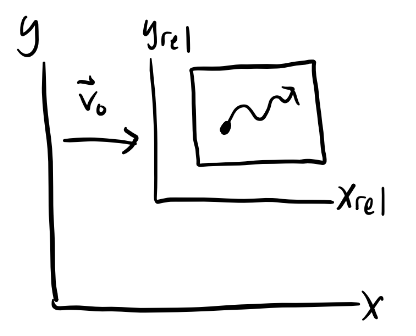
\includegraphics[width=2.60417in,height=\textheight]{classical-mechanics/./resources/image-20230216114604959.png}

}

\end{figure}

Evidently, \(\mathbf{x} = \mathbf{x}_{rel} + \mathbf{v}_0t\), which
means \(\mathbf{v} = \mathbf{v}_{rel} + \mathbf{v}_0\), and
\(\mathbf{a} = \mathbf{a}_{rel} + \mathbf{a}_0\). When
\(\mathbf{a}_0=\mathbf{0}\) we recover the special case of a
\textbf{Galilean transformation}. In that case,
\(\mathbf{F} = m \mathbf{a} = m \mathbf{a}_{rel}\), which means
\(S_{rel}\) is by definition an inertial frame.

If \(\mathbf{a}_0 \neq \mathbf{0}\), we get
\(\mathbf{F} = m(\mathbf{a}_0 + \mathbf{a}_{rel})\), or
\(m\mathbf{a}_{rel} = \mathbf{F} - m \mathbf{a}_0\). We can think about
this in another way, by defining a relative force
\(\mathbf{F}_{rel} = m\mathbf{a}_{rel}\) and thinking of it as being
composed of an \emph{inertial} force \(\mathbf{F}\) along with a
\emph{fictitious} force \(\mathbf{F}_{lin} = -m\mathbf{a}_0\), \[
\mathbf{F}_{rel} = \mathbf{F} + \mathbf{F}_{lin} = \mathbf{F} - m \mathbf{a}_0.
\] One special case of a linear accelerating frame is an object
free-falling under gravity. In that case, \(\mathbf{a}_0=-\mathbf{g}\)
is constant. In some sense, this means we can treat gravity as a kind of
generalized coordinate transformation that shifts the acceleration from
\(\mathbf{a}\) to \(\mathbf{a}_{rel} = \mathbf{a} + \mathbf{g}\). This
curious fact arises due to the \textbf{equivalence principle}, which
says the gravitational force is proportional to the inertial mass \(m\).
This curious fact causes the \(m\) to cancel from both sides of
\(m\mathbf{a} = m\mathbf{g}\). As far as we know, gravity is the
\emph{only} force in nature with this special property. The equivalence
principle is essentially the launch point to Einstein's general theory
of relativity.

\begin{figure}

{\centering 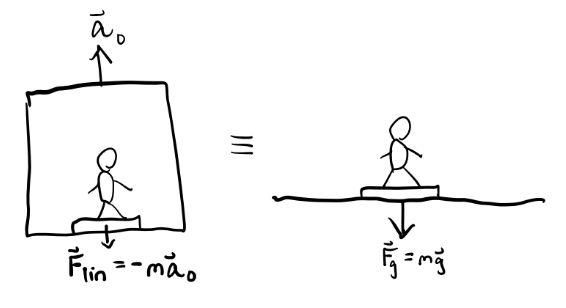
\includegraphics[width=4.16667in,height=\textheight]{classical-mechanics/./resources/image-20230217104903472.png}

}

\end{figure}

\hypertarget{example-pendulum-in-an-accelerating-railcar}{%
\subsection{Example: Pendulum in an accelerating
railcar}\label{example-pendulum-in-an-accelerating-railcar}}

A railcar is moving along the x-axis at a constant acceleration
\(\mathbf{a}_0\) with respect to the lab frame. Inside the railcar, a
pendulum with mass \(m\) and length \(\ell\) is attached to the ceiling
and allowed to swing freely. Find the equations of motion for the
swinging pendulum. Also, find the equilibrium position of the pendulum.

\begin{figure}

{\centering 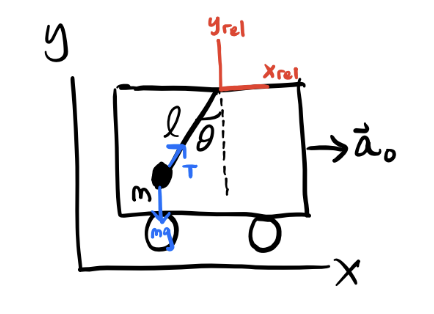
\includegraphics[width=3.125in,height=\textheight]{classical-mechanics/./resources/image-20230217105357519.png}

}

\end{figure}

Working in the frame of the railcar, we have
\(\mathbf{F}_{rel} = \mathbf{F} + \mathbf{F}_{lin}\). The inertial
forces on the pendulum are the string tension \(\mathbf{T}\) and gravity
\(m\mathbf{g}\). We thus have \[
m\mathbf{a}_{rel} = \mathbf{T} + m\mathbf{g} - m\mathbf{a}_0 \equiv \mathbf{T} + m\mathbf{g}_{eff},
\] where \(\mathbf{g}_{eff} \equiv \mathbf{g} - \mathbf{a}_0\) acts as
an \emph{effective gravity} on the pendulum inside the moving railcar.
We can thus use the standard method to solve for the pendulum, but
replacing \(\mathbf{g}\) with \(\mathbf{g}_{eff}\), to get \[
\ddot \theta = -\omega^2 \sin \theta, \quad \text{where} \quad \omega^2 \equiv \frac{|\mathbf{g}_{eff}|}{\ell} = \frac{\sqrt{g^2 + a_0^2}}{\ell}.
\] The equilibrium position occurs when \(\mathbf{F}_{rel}=\mathbf{0}\),
which is when \(\mathbf{T} = -m\mathbf{g}_{eff}\). Using a little trig,
we can see the equilibrium angle will be shifted to the angle
\(\theta_{eq}\) given by

\begin{figure}

{\centering 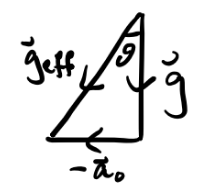
\includegraphics[width=1.45833in,height=\textheight]{classical-mechanics/./resources/image-20230217110859846.png}

}

\end{figure}

\[
\theta_{eq} = \tan^{-1} \frac{g}{a_0}.
\]

Notice when \(a_0\) we get \(\theta_{eq}=0\), which is what we'd expect
if the railcar weren't accelerating.

\hypertarget{rotating-frames}{%
\section{Rotating Frames}\label{rotating-frames}}

Let's now look at reference frames that are rotating about some axis.
Without loss of generality, we'll consider a reference frame \(S_{rot}\)
that's rotating about the z-axis with respect to the lab frame \(S\) at
some angular velocity
\(\boldsymbol{\omega} = \dot \varphi \mathbf{e}_z\).

\begin{figure}

{\centering 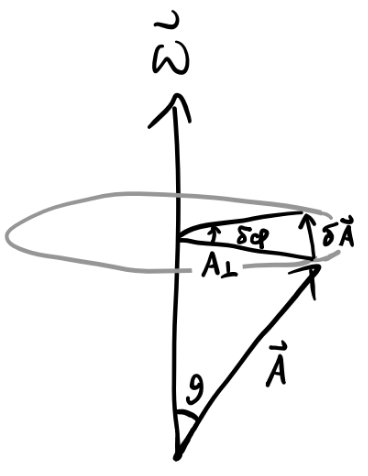
\includegraphics[width=2.08333in,height=\textheight]{classical-mechanics/./resources/image-20230217111757574.png}

}

\end{figure}

Let \(\mathbf{A}\) be some vector in this rotating frame that's at an
angle \(\theta\) with the axis of rotation. The amount that
\(\mathbf{A}\) changes due to the frame's rotation by an amount
\(\delta\varphi\) is given by \[
\delta A = A_\perp \delta\varphi = A\sin\theta\delta\varphi = |\mathbf{A} \times \delta\boldsymbol{\varphi}|,
\] so by the right-hand rule we have
\(\delta\mathbf{A} = \delta\boldsymbol{\varphi} \times \mathbf{A}\).
Dividing both sides by \(dt\), we finally have \[
\frac{d\mathbf{A}}{dt} = \boldsymbol{\omega} \times \mathbf{A}.
\] \textbf{Remark: } Since velocities add as vectors, so too do angular
velocities. This means if \(S'\) is a frame rotating relative \(S\), and
\(S''\) is yet \emph{another} frame that's rotating to \(S'\), then we
have \[
\mathbf{v}_S'' = \mathbf{v}_S' + \mathbf{v}_{S'}'' \quad \Longrightarrow \quad  \boldsymbol{\omega}_S'' \times \mathbf{r}_S = \boldsymbol{\omega}' \times \mathbf{r}_S + \boldsymbol{\omega}'' \times \mathbf{r}_{S'} \quad \Longrightarrow \quad  \boldsymbol{\omega}_S'' = \boldsymbol{\omega}_S' + \boldsymbol{\omega}_{S'}''.
\] This fact allows us to easily solve problems involving complex
hierarchies of rotations.

Now, suppose \(S_{rot}\) is rotating with angular velocity
\(\boldsymbol{\omega}\) with respect to the origin of \(S\). With
respect to an observer in each frame, a vector
\(\mathbf{A} = A_i \mathbf{e}_i = A_i^{rot}\mathbf{e}_i = \mathbf{A}_{rel}\)
changes as

\[
\begin{align*}
\frac{d\mathbf{A}}{dt}\bigg|_{rot} &= \dot A_i^{rot} \mathbf{e}_i^{rot}, \\
\frac{d\mathbf{A}}{dt}\bigg|_{lab} &= \dot A_i^{rot} \mathbf{e}_i^{rot} + A_i^{rot} \mathbf{\dot e}_i^{rot}, \\
\frac{d\mathbf{e}_i^{rot}}{dt}\bigg|_{lab} &= \boldsymbol{\omega} \times \mathbf{e}_i^{rot}.
\end{align*}
\] Thus, we have \[
\frac{d\mathbf{A}}{dt}\bigg|_{lab} = \frac{d\mathbf{A}}{dt}\bigg|_{rot} + \boldsymbol{\omega} \times \mathbf{A}_{rot}
\] This evidently defines a \emph{transport} operation between the lab
frame and the rotating frame. Namely, time derivatives in the lab frame
are related to time derivatives in the rotating frame via \[
\frac{d}{dt}\bigg|_{lab} = \frac{d}{dt}\bigg|_{rot} + \boldsymbol{\omega} \times.
\] This result is sometimes called the \textbf{transport theorem}.

Using the transport theorem we can now derive what the equations of
motion look like inside the rotating frame. Plugging \(\mathbf{x}\) into
the transport equation, we get \[
\frac{d\mathbf{x}}{dt}\bigg|_{lab} = \frac{d\mathbf{x}}{dt}\bigg|_{rot} + \boldsymbol{\omega} \times \mathbf{x}_{rot},
\] or \[
\mathbf{v} = \mathbf{v}_{rot} + \boldsymbol{\omega} \times \mathbf{x}_{rot}.
\] To get the acceleration \(\mathbf{a}\), we need to apply the
transport equation \emph{again} to the velocity vector,

\[
\begin{align*}
\frac{d\mathbf{v}}{dt}\bigg|_{lab} &= \bigg(\frac{d}{dt}\bigg|_{rot} + \boldsymbol{\omega} \times \bigg) (\mathbf{v}_{rot} + \boldsymbol{\omega} \times \mathbf{x}_{rot}) \\
&= \mathbf{\dot v}_{rot} + \boldsymbol{\omega} \times \mathbf{v}_{rot} + \boldsymbol{\dot \omega} \times \mathbf{x}_{rot} + \boldsymbol{\omega} \times \mathbf{v}_{rot} + \boldsymbol{\omega} \times (\boldsymbol{\omega} \times \mathbf{x}_{rot}).
\end{align*}
\] Or after cleaning up a bit, \[
\mathbf{a} = \mathbf{a}_{rot} + 2 \boldsymbol{\omega} \times \mathbf{v}_{rot} + \boldsymbol{\dot \omega} \times \mathbf{x}_{rot} + \boldsymbol{\omega} \times (\boldsymbol{\omega} \times \mathbf{x}_{rot}).
\]

Since \(\mathbf{F} = m \mathbf{a}\) in the lab frame, we can multiply
both sides by \(m\) and re-arrange terms to get the force vector
\(\mathbf{F}_{rot}\), \[
\mathbf{F}_{rot} = \mathbf{F} + m \boldsymbol{\omega} \times (\mathbf{x}_{rot} \times \boldsymbol{\omega}) + 2m \mathbf{v}_{rot} \times \boldsymbol{\omega} + m \mathbf{x}_{rot} \times \boldsymbol{\dot \omega}.
\] Evidently, there are three distinct fictitious force terms.
Naturally, they each have special names:

\begin{itemize}
\tightlist
\item
  Centrifugal Force:
  \(\mathbf{F}_{cf} = m \boldsymbol{\omega} \times (\mathbf{x}_{rot} \times \boldsymbol{\omega}) = m(\boldsymbol{\omega} \cdot \mathbf{x}_{rot})\mathbf{x}_{rot} - m\omega^2 \mathbf{x}_{rot}\).
\item
  Coriolis Force:
  \(\mathbf{F}_{cor} = 2m \mathbf{v}_{rot} \times \boldsymbol{\omega}\).
\item
  Euler Force:
  \(\mathbf{F}_{eul} = m \mathbf{x}_{rot} \times \boldsymbol{\dot \omega}\).
\end{itemize}

In terms of these forces, we can finally write the force experienced in
the rotating frame as \[
\mathbf{F}_{rot} = \mathbf{F} + \mathbf{F}_{cf} + \mathbf{F}_{cor} + \mathbf{F}_{eul}.
\] The centrifugal force tends to push a rotating object outward
radially from the origin, similar to how a centrifuge works. In the
simple case when the position is perpendicular to the axis of rotation,
the centrifugal force reduces to the more familiar form from elementary
physics, \[
\mathbf{F}_{cf} = - m\omega^2 \mathbf{x}_{rot} = -\frac{mv_{rot}^2}{r_{rot}} \mathbf{e}_r.
\] The Coriolis force tends to deflect a moving object away from its
line of motion. It arises due to the fact that as the object moves, the
frame under it is rotating underneath, which causes an apparent
deflection sideward.

\hypertarget{example-throwing-a-baseball-from-the-north-pole}{%
\subsection{Example: Throwing a baseball from the North
Pole}\label{example-throwing-a-baseball-from-the-north-pole}}

Suppose a baseball is thrown from the North Pole for a distance \(\ell\)
and a constant velocity \(\mathbf{v}_0\) with respect to the lab frame.
Find the deflection angle \(\delta\theta\) of the ball caused by the
Coriolis force.

\begin{figure}

{\centering 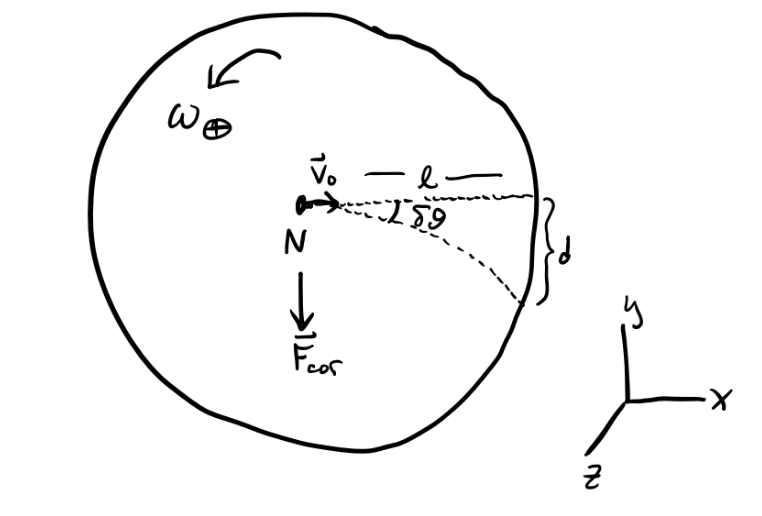
\includegraphics[width=4.16667in,height=\textheight]{classical-mechanics/./resources/image-20230217134747801.png}

}

\end{figure}

The rotating frame in this case is the Earth itself. The Earth rotates
counterclockwise about the North Pole with an angular velocity of
\(\omega_\oplus = \frac{2\pi}{\text{1 day}} \approx 7 \cdot 10^{-5} \frac{\text{rad}}{\text{sec}}\).
Suppose \(\mathbf{e}_z\) is the direction pointing \emph{skyward}, with
the origin at the North Pole. Then
\(\boldsymbol{\omega} = \omega_{\oplus} \mathbf{e}_z\). Suppose the ball
is thrown initially along the positive x-axis, so
\(\mathbf{x} = \ell \mathbf{e}_x\). Since
\(\mathbf{v} = \mathbf{v}_{rot} + \boldsymbol{\omega} \times \mathbf{x}_{rot}\),
we have \[
\mathbf{v}_0 = \mathbf{v}_{rot} + \omega_{\oplus} v_0 t (\mathbf{e}_z \times \mathbf{e}_x) = \mathbf{v}_{rot} + \omega_{\oplus} v_0 t \mathbf{e}_y.
\] On time scales \(t \ll \text{1 day}\), we can say
\(\mathbf{v}_{rot} \approx \mathbf{v}_0\) since in that case
\(\omega_{\oplus} t\) becomes small. Then we have \[
\mathbf{F}_{cor} = 2m \mathbf{v}_{rot} \times \boldsymbol{\omega} \approx 2m v_0 \omega_{\oplus} (\mathbf{e}_x \times \mathbf{e}_z) = -2m v_0 \omega_{\oplus} \mathbf{e}_y,
\] Evidently, the Coriolis force in this case is constant, which means
the acceleration \(\mathbf{a}_{cor}\) is constant too. We thus get a
simple constant equation of motion in \(y\), \[
\ddot y = -2v_0 \omega_{\oplus}.
\] Solving this EOM gives a deflection distance of \[
d = |y| = \frac{1}{2}(2v_0 \omega_{\oplus})^2 = v_0 \omega_{\oplus} t^2.
\] Finally, we can use this to calculate the deflection angle
\(\delta\theta\), \[
\delta\theta \approx \frac{d}{\ell} = \frac{\omega_{\oplus}v_0 t^2}{v_0 t} = \omega_{\oplus} t.
\] To plug in some numbers, suppose the ball stays in the air for
\(t = \text{100 sec}\). Then we'd get
\(\delta\theta \approx 0.4^\circ\), indeed a very small deflection.

\hypertarget{example-hurricanes}{%
\section{Example: Hurricanes}\label{example-hurricanes}}

It turns out that hurricanes rotate the direction they do due to the
Coriolis force of the Earth. Pressure gradients cause water currents
flowing east-west to spiral inward. In the Northern hemisphere, water
deflects rightward, causing the gradients (or ``hurricanes'') to spiral
counterclockwise. Whereas in the Southern hemisphere, water deflects
leftward, causing gradients (or ``typhoons'') to spiral clockwise.

\begin{figure}

{\centering 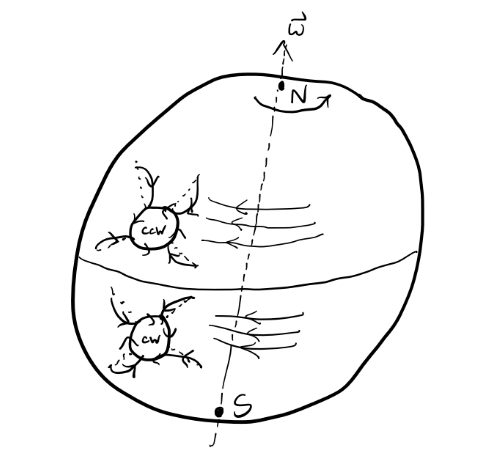
\includegraphics[width=3.125in,height=\textheight]{classical-mechanics/./resources/image-20230217142823695.png}

}

\end{figure}

\hypertarget{example-the-foucalt-pendulum}{%
\section{Example: The Foucalt
pendulum}\label{example-the-foucalt-pendulum}}

The Foucalt pendulum is a classic problem that's often used to
demonstrate that the Earth rotates. Suppose a very long pendulum of
length \(l\) and mass \(m\) is fixed near the Earth's surface at some
latitude \(\lambda\) above the equator. Here's a picture of what's going
on.

\begin{figure}

{\centering 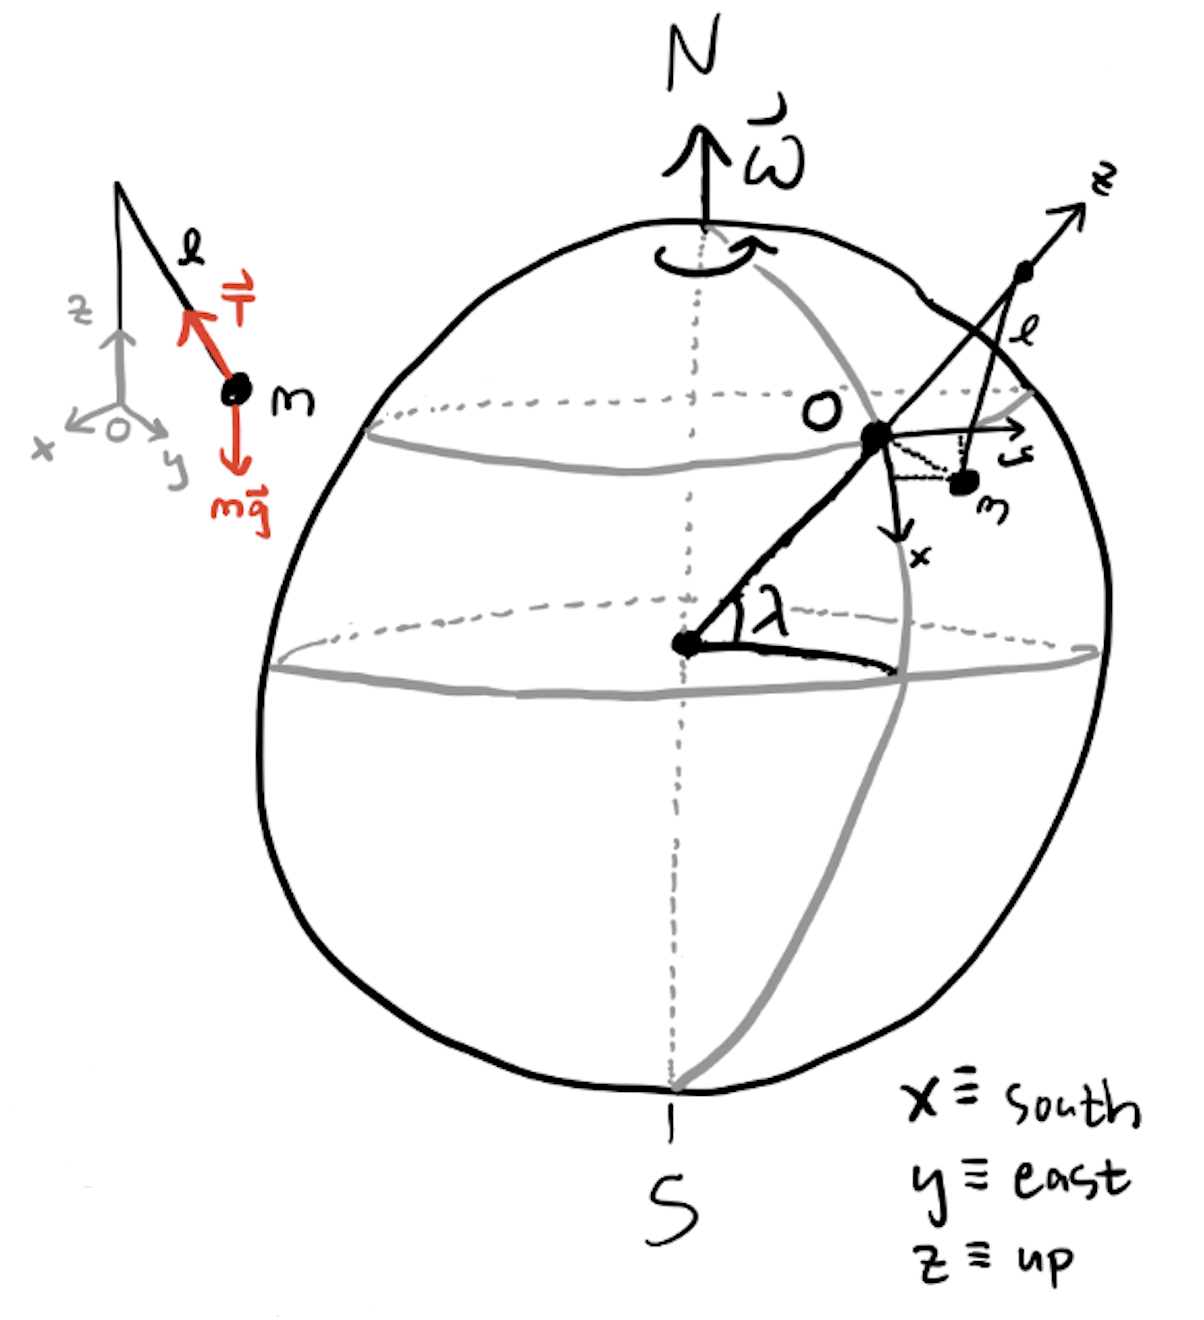
\includegraphics[width=4.16667in,height=\textheight]{classical-mechanics/./resources/image-20230217145604558.png}

}

\end{figure}

It's reasonable to assume that \(\omega_{\oplus}\) is constant, so the
Euler force is zero. It's also reasonable to assume the centrifugal
force is zero since \(\omega_{\oplus}\) is small. Thus, in the frame of
the rotating Earth, we're left with the inertial forces on the pendulum
and the Coriolis force, \[
m\mathbf{a}_{rot} = m\mathbf{g} + \mathbf{T} - 2m\boldsymbol{\omega} \times \mathbf{v}_{rot}.
\] Choose the axes such that the z-axis is pointing outward from the
Earth's surface at the pendulum and the other axes are planar to the
surface. Now, we can write \(\mathbf{g} = -g \mathbf{e}_z\), and using
some trig it's not too hard to show that \[
\mathbf{T} \approx -\frac{T}{\ell} (x \mathbf{e}_x + y \mathbf{e}_y + \ell \mathbf{z}).
\] Using the latitude angle \(\lambda\) we can also express the angular
velocity \(\boldsymbol{\omega}\) as \[
\boldsymbol{\omega} = -\omega_{\oplus}\cos\lambda\mathbf{e}_x + \omega_{\oplus}\sin\lambda\mathbf{e}_z.
\] Since the pendulum approximately speaking only moves in the xy-plane,
we also have \[
\mathbf{v}_{rot} = \dot x \mathbf{e}_x + \dot y \mathbf{e}_y.
\] Together, these together imply \[
\boldsymbol{\omega} \times \mathbf{v}_{rot} \approx -\dot y \omega_{\oplus} \sin\lambda \mathbf{e}_x + \dot x \omega_{\oplus} \sin\lambda \mathbf{e}_y - \dot y \omega_{\oplus} \cos\lambda \mathbf{e}_z.
\] This means \[
\mathbf{a}_{rot} = \bigg(-\frac{Tx}{m\ell} + 2\dot y \omega_{\oplus} \sin\lambda \bigg) \mathbf{e}_x + \bigg(-\frac{Ty}{m\ell} - 2\dot x \omega_{\oplus} \sin\lambda \bigg) \mathbf{e}_x,
\] which gives equations of motion

\[
\begin{align*}
\ddot x &= -\frac{T}{m\ell} \cdot x + 2\omega_{\oplus}\sin\lambda \cdot \dot y \\
\ddot y &= -\frac{T}{m\ell} \cdot y - 2\omega_{\oplus}\sin\lambda \cdot \dot x. \\
\end{align*}
\] If we define \(\omega_0^2 \equiv \frac{T}{m\ell} = \frac{g}{\ell}\),
we can re-arrange and write the equations of motion in the form

\[
\begin{align*}
\ddot x + \omega_0^2 \cdot x &= 2\omega_z \dot y \\
\ddot y + \omega_0^2 \frac{T}{m\ell} \cdot y &= -2\omega_z \dot x, \\
\end{align*}
\] where \(\omega_z = \omega_{\oplus}\sin\lambda\). If we combine these
two equations, this is equivalent to a complex DHO problem with
imaginary damping, \[
\ddot z + 2i\omega_z \dot z + \omega_0^2 z = 0.
\] This means solutions will have the form \[
z(t) = e^{-i\omega_z t}(A e^{i\omega't} + B e^{-i\omega't}).
\] where \(\omega' \equiv \sqrt{\omega_z^2 + \omega_0^2}\). If we assume
the pendulum swings much faster than the Earth rotates, we have
\(\omega_0 \gg \omega_{\oplus}\), which means we can approximate
\(z(t)\) as \[
z(t) \approx e^{-i\omega_z t}(A e^{i\omega_0 t} + B e^{-i\omega_0 t}).
\] If we define \(z'(t) \equiv A e^{i\omega_0 t} + B e^{-i\omega_0 t}\),
then \(z(t) = e^{-i\omega_z t} z'(t)\), and we can write the real
solutions as

\[
\begin{align*}
x(t) &= x'(t) \cos\omega_z t + y'(t) \sin\omega_z t, \\
y(t) &= -x'(t) \sin\omega_z t + y'(t) \cos\omega_z t. \\
\end{align*}
\] This says that the plane of oscillation itself undergoes a rotation
in the xy-plane. That is, the plane of the pendulum's orbit
\emph{precesses} with a frequency given by \[
\omega_z = \omega_{\oplus} \sin\lambda = 2\pi\frac{\sin\lambda}{\text{1 day}}.
\] For example, at a latitude of \(\lambda = 34.5^\circ\), the pendulum
precesses counterclockwise with a frequency of
\(\omega_z \approx \text{3.86 rad/sec}\), or about \(8.5^\circ\) per
hour. It appears precession is non-existent at the equator and highest
at the poles, where precession happens exactly with the Earth's
rotation.

\hypertarget{general-non-inertial-frames}{%
\section{General Non-Inertial
Frames}\label{general-non-inertial-frames}}

More generally, we can combine linearly accelerating and rotating frames
by just adding the fictitious forces together. If \(S_{rel}\) is both
accelerating and rotating about some axis with respect to \(S\), we'd
have \[
\mathbf{F}_{rel} = \mathbf{F} + \mathbf{F}_{lin} + \mathbf{F}_{cf} + \mathbf{F}_{cor} + \mathbf{F}_{eul}.
\] This general form for a force in a non-inertial frame can be used to
analyze a surprisingly large number of practical problems, where
complicated forces can often be decomposed into a sum of linear forces
and rotational forces.

One fact to be aware of about non-inertial frames is that energy need
not be conserved. It's only true in inertial frames that energy must be
conserved. This has to do with the fact that in the relative frame we're
ignoring the forces on the relative frame itself, i.e.~the forces that
cause the frame to accelerate or rotate. We can generally recover the
conservation of energy by transforming back to an inertial frame.

\hypertarget{lagrangian-mechanics}{%
\chapter{Lagrangian Mechanics}\label{lagrangian-mechanics}}

While Newton's Laws give a complete description of classical mechanics,
they can be cumbersome to apply when complicated forces are present.
Lagrangian mechanics is an alternative but completely equivalent
approach to Newtonian mechanics that greatly simplifies many problems,
particularly where constraint forces are present. Not only that, but
unlike Newtonian mechanics, the Lagrangian formulation can be extended
to many other areas of physics, including quantum mechanics and general
relativity.

\hypertarget{configuration-space}{%
\section{Configuration Space}\label{configuration-space}}

Many forces acting on a system do no work. They serve only to keep
particles confined to some surface in space. Such forces are called
\textbf{forces of constraint}. Examples of forces of constraint include
the tension in a string and the normal force keeping an object on a
physical surface.

Suppose we have a system of \(N\) particles with positions
\(\mathbf{x}_1, \mathbf{x}_2, \cdots, \mathbf{x}_N\) respectively. Taken
together, these positions can be thought of as defining a trajectory in
the \(3N\)-dimensional space \(\mathbb{R}^{3N}\). A \textbf{holonomic
constraint} is a constraint that keeps the \(N\) particles confined to
some lower-dimensional sub-manifold \(\mathcal{Q}\) of
\(\mathbb{R}^{3N}\). Equivalently, it's a (possibly time-dependent)
function of the form \[
f(\mathbf{x}_1, \mathbf{x}_2, \cdots, \mathbf{x}_N, t) = 0.
\] The dimension of \(\mathcal{Q}\) is \(n=3N-C\), where \(C\) is the
total number of constraints on the system. These are the number of
\textbf{degrees of freedom} of the system. This sub-manifold is called
the \textbf{configuration space} of the system. Since \(\mathcal{Q}\) is
\(n\)-dimensional, we should be able to parametrize it with \(n\)
coordinates \(q_1, q_2, \cdots, q_n\). We call these \textbf{generalized
coordinates}. They're not ordinary coordinates in real space. They're a
way of describing where in configuration space the system is at a given
point in time.

\begin{figure}

{\centering 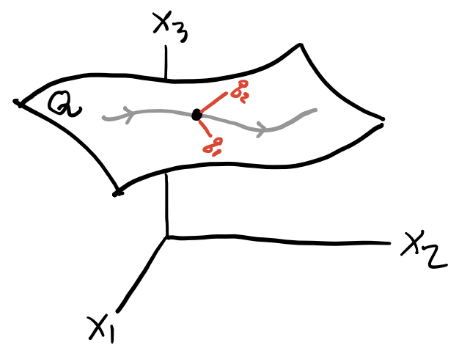
\includegraphics[width=3.125in,height=\textheight]{classical-mechanics/./resources/image-20230218194924026.png}

}

\end{figure}

Holonomicity requires that we be able to find a 1-1 map going back and
forth between generalized coordinates and the position vectors, \[
q_i = q_i(\mathbf{x}_1, \mathbf{x}_2, \cdots, \mathbf{x}_N, t), \quad \mathbf{x}_\alpha = \mathbf{x}_\alpha(q_1, q_2, \cdots, q_n, t).
\] When the holonomic constraint isn't time-dependent, they're called
\textbf{scleronomic} constraints. Otherwise they're called
\textbf{rheonomic} constraints. A system that's not holonomic is called
\textbf{non-holonomic}.

As an easy example, consider the simple pendulum. Since there's only one
particle, \(N=1\). Since the length of the pendulum is fixed, that's one
constraint. Since the motion is confined to a plane, that's another
constraint. We thus have \(n=3N-C=3-2=1\) degrees of freedom, which we
can of course take to be the angle \(\theta\).

A more interesting example is the rigid body. A \textbf{rigid body} is a
system of \(N\) particles whose particles are always a fixed distance
apart, i.e.~\(d_{ij} = |\mathbf{x}_i - \mathbf{x}_j|\) is fixed for all
\(i, j\). This fixed distance requirement introduces a lot of
constraints on the system. To see this, suppose \(N=4\). Then there are
\(C=6\) constraints, since each particle must connect to each other
particle. This means there are \(n=3N-C=6\) degrees of freedom.

\begin{figure}

{\centering 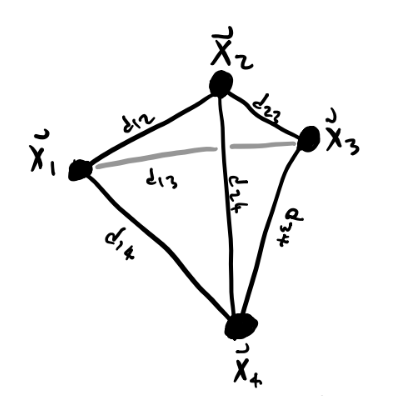
\includegraphics[width=2.08333in,height=\textheight]{classical-mechanics/./resources/image-20230218201852629.png}

}

\end{figure}

It turns out this fact extends to rigid bodies with arbitrarily many
particles as well since adding a new particle gives 3 more coordinates,
but also 3 more constraints. A rigid body will \emph{always} have
exactly 6 degrees of freedom, which we usually take to be the 3 center
of mass coordinates and the three Euler angles.

\hypertarget{virtual-work}{%
\section{Virtual Work}\label{virtual-work}}

Suppose we have a system of \(N\) particles in mechanical equilibrium,
so \(\mathbf{F}_i=\mathbf{0}\) for all \(i\). Let's imagine we perturb
each particle \(\mathbf{x}_i\) by some amount \(\delta \mathbf{x}_i\),
but only in a way that doesn't change the configuration space. This
means each perturbation must be a function of the generalized
coordinates,
\(\delta \mathbf{x}_i = \delta \mathbf{x}_i(q_1, q_2, \cdots, q_n, t)\).
Define the \textbf{virtual work} done on the system by, \[
\delta W \equiv \sum \mathbf{F}_i \cdot \delta\mathbf{x}_i
\] Now, let's decompose each force \(\mathbf{F}_i\) into a sum of two
components, an \emph{applied force} \(\mathbf{F}_i^{app}\) and a
constraint force \(\mathbf{F}_i^{con}\). The applied forces are the ones
that do work on each particle, while the constraint forces are the ones
that keep them confined to the configuration space. If the system is
exactly in equilibrium, then
\(\mathbf{F}_i = \mathbf{F}_i^{app} + \mathbf{F}_i^{con} = \mathbf{0}\),
which means \(\delta W = 0\) in equilibrium. But since constraint forces
do no work, we get \[
\delta W = \sum \mathbf{F}_i^{app} \cdot \delta\mathbf{x}_i = 0
\] This is called the \textbf{principle of virtual work}.

\textbf{Note:} Sometimes constraint forces \emph{do} in fact do work on
a system. One major example is a system in rolling motion, e.g.~a wheel
rolling down a ramp. We'll mostly ignore these situations in this
lesson.

More generally, if a system is not in equilibrium, we have
\(\mathbf{F}_i = m_i \mathbf{\dot v}_i\). If we insist the principle of
virtual work must apply to these situations as well, we have \[
\begin{align*}
0 = \delta W &= \sum_i (\mathbf{F}_i^{app} - m_i \mathbf{\dot v}_i) \cdot \delta \mathbf{x}_i \\
&= \sum_i (\mathbf{F}_i^{app} - m_i \mathbf{\dot v}_i) \cdot \sum_j\frac{\partial \mathbf{x}_i}{\partial q_j} \delta q_j \\
&= \sum_j \bigg(\sum_i \mathbf{F}_i^{app} \cdot \frac{\partial \mathbf{x}_i}{\partial q_j}  - m_i \mathbf{\dot v}_i \cdot \frac{\partial \mathbf{x}_i}{\partial q_j} \bigg) \delta q_j \\
&= \sum_j \bigg[ Q_j - \bigg(\frac{d}{dt} \frac{\partial T}{\partial \dot q_j} - \frac{\partial T}{\partial q_j} \bigg) \bigg] \delta q_j.
\end{align*}
\] Here I defined
\(Q_j \equiv \mathbf{F}_i^{app} \cdot \frac{\partial \mathbf{x}_i}{\partial q_j}\).
This term is called the \textbf{generalized force}. It acts as a force,
but on the generalized coordinates instead of the position vectors
directly. The other thing I did was re-wrote the momentum term by using
the total kinetic energy \(T = \frac{1}{2} \sum_i m_i \mathbf{v}_i^2\).
Now, if we insist that all the \(q_i\) are independent of each other,
then the terms in the sum must vanish individually, which means for all
\(j=1,\cdots,n\) we have \[
Q_j = \frac{d}{dt} \frac{\partial T}{\partial \dot q_j} - \frac{\partial T}{\partial q_j}.
\] In the special case where the forces on the system are conservative,
we can use the potential energy \(V\) to express the generalized forces
as \(Q_j = -\frac{\partial V}{\partial q_i}\). Defining a function
\(L \equiv T - V\) called the \textbf{Lagrangian} and re-arranging
terms, we finally have \[
\frac{\partial L}{\partial q_j} - \frac{d}{dt} \frac{\partial L}{\partial \dot q_j} = 0.
\] This gives a set of \(n\) equations for the generalized coordinates,
called \textbf{Lagrange's equations}.

To see why the Lagrange's equations are useful, consider the special
case where \(T=\frac{1}{2} \sum_i m_i \dot x_i^2\) and
\(V = V(x_1, x_2, \cdots, x_n)\). Then we have a Lagrangian of the form
\[
L = T - V = \frac{1}{2} \sum_i m_i \dot x_i^2 - V(x_1, x_2, \cdots, x_n),
\] which we can plug into the Euler-Lagrange Equations to get \[
m \ddot x_i = - \frac{\partial V}{\partial x_i} \quad \forall i=1,2,\cdots,n.
\] But this is just \(\mathbf{F} = m \mathbf{a}\)! Evidently we've
managed to reproduce Newton's Laws from Lagrange's equations. This in
some sense suggest that Lagrange's equations might be more general than
Newton's Laws, and in fact they are as we'll see later.

\hypertarget{examples-1}{%
\section{Examples}\label{examples-1}}

The Lagrangian formulation is very useful for solving problems that
would be very complicated to solve using Newtonian approaches. This is
particular true when there are complex constraints present. It's thus
very helpful to see a bunch of examples showing how to solve problems
using Lagrangian methods.

To solve a problem using Lagrange's equations we need to do the
following steps:

\begin{enumerate}
\def\labelenumi{\arabic{enumi}.}
\tightlist
\item
  Figure out how many degrees of freedom the system has using
  \(n=3N-C\).
\item
  Identify the generalized coordinates \(q_1,q_2,\cdots,q_n\).
\item
  Express each of the velocity vectors as a function of the \(q_i\)'s,
  \(\mathbf{v}_i = \mathbf{v}_i(q_1,q_2,\cdots,q_n)\). Use these to
  write down the kinetic energy as
  \(T = \frac{1}{2}\sum_i m_i \mathbf{v_i}^2\).
\item
  Write down the potential energy as a function of the \(q_i\)'s, so
  \(V=V(q_1,q_2,\cdots,q_n)\).
\item
  Write down the Lagrangian \(L = T - V\).
\item
  Use Lagrange's equations to get the equations of motion for the
  \(q_i\)'s.
\item
  Solve for the trajectories \(q_1(t),q_2(t),\cdots,q_n(t)\).
\item
  If desired, convert back to real space coordinates via
  \(\mathbf{x}_\alpha = \mathbf{x}_\alpha(q_1,q_2,\cdots,q_n)\).
\end{enumerate}

\hypertarget{example-the-simple-spring}{%
\subsubsection{Example: The Simple
Spring}\label{example-the-simple-spring}}

Suppose a mass \(m\) is attached to an ideal spring with spring constant
\(k\).

\begin{figure}

{\centering 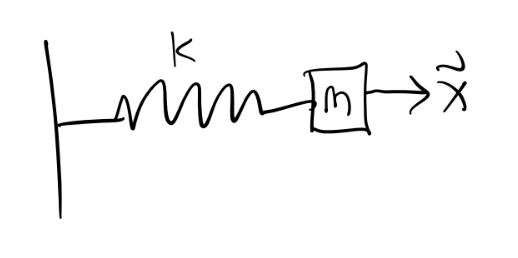
\includegraphics[width=3.125in,height=\textheight]{classical-mechanics/./resources/image-20230218211506460.png}

}

\end{figure}

In this case, \(N = 1\), and the spring is constrained to move along,
say, the x-axis, so \(C=2\), and there's just \(n=3N-C=1\) degree of
freedom (as expected). If the generalized coordinate is just \(q=x\), we
have \[
T = \frac{1}{2} m \dot q^2, \quad V = \frac{1}{2}kq^2,
\] which means the Lagrangian is \[
L = \frac{1}{2} m \dot q^2 - \frac{1}{2}kq^2.
\] Solving Lagrange's equation in this case gives \[
-\frac{\partial}{\partial q} \frac{k q^2}{2} - \frac{d}{dt} \frac{\partial}{\partial \dot q} \frac{m\dot q^2}{2} = 0 \quad \Rightarrow \quad m\ddot q = -k q.
\] We've already seen the solution to this equation is just the SHO
solution \[
q(t) = A\cos(\omega t - \delta), \quad \omega^2 \equiv \frac{k}{m}.
\] If desired, in this case we could convert back to real coordinates
via \[
\mathbf{x}(t) = q(t) \mathbf{e}_x = A\cos(\omega t - \delta)\mathbf{e}_x.
\]

\hypertarget{example-simple-pendulum-1}{%
\subsubsection{Example: Simple
Pendulum}\label{example-simple-pendulum-1}}

Suppose a mass \(m\) is attached to a massless string of fixed length
\(\ell\) and allowed to swing.

\begin{figure}

{\centering 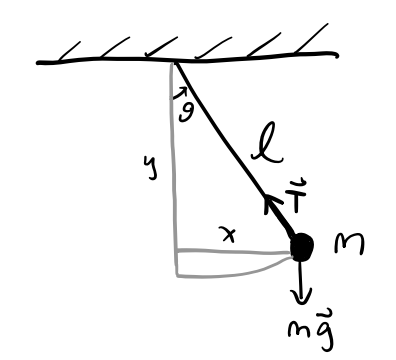
\includegraphics[width=3.125in,height=\textheight]{classical-mechanics/./resources/image-20230212040128210.png}

}

\end{figure}

In this problem, there's \(N=1\) particle. The string being fixed adds
one constraint, and motion being confined to the plane adds another, so
we have \(n=1\) degrees of freedom here, which we'll take to be the
angle \(q=\theta\). Using polar coordinates, we can write the kinetic
and potential energies as \[
T = \frac{1}{2} m\ell^2 \dot q^2, \quad V = -mg\ell\cos q,
\] which gives a Lagrangian \[
L = \frac{1}{2} m\ell^2 \dot q^2 + mg\ell\cos q.
\] Solving Lagrange's equation, we get the equation of motion \[
m\ell^2 \ddot q + mg\ell\sin q = 0,
\] which is of course the usual equation of motion for the pendulum when
\(q=\theta\).

\hypertarget{example-central-potential}{%
\subsubsection{Example: Central
Potential}\label{example-central-potential}}

Suppose a particle of mass \(m\) is in the presence of a central force
field \(V=V(r)\). There's one constraint since the problem must be
spherically symmetric, which means we have \(n=2\) degrees of freedom.
Working in spherical coordinates, the kinetic and potential energies are
given by \[
T = \frac{1}{2} m (\dot r^2 + r \dot \varphi^2), \quad V = V(r).
\] Plugging these into Lagrange's equation and solving gives two
equations of motion for \(r\) and \(\varphi\), \[
m \ddot r = mr \dot\varphi^2 - \frac{dV}{dr}\\
\frac{d}{dt} mr^2 \dot\varphi = 0.
\] The second equation is interesting. It says the quantity
\(\ell = mr^2 \dot\varphi\) must be conserved. But this is just the
angular momentum of the system! Evidently, conservation laws somehow
fall out of Lagrange's equations provided the right generalized
coordinates are chosen.

\hypertarget{example-double-pendulum}{%
\subsubsection{Example: Double Pendulum}\label{example-double-pendulum}}

The examples considered so far are pretty easy to solve using Newtonian
methods. Here's an example that's far easier to solve in the Lagrangian
formulation. Suppose we have a double pendulum, where a mass is attached
to the end of another pendulum and both are allowed to swing. Suppose
both masses have mass \(m\) and both strings are a fixed length
\(\ell\).

\begin{figure}

{\centering \includegraphics[width=3.125in,height=\textheight]{classical-mechanics/./resources/image-20230218215415855.png}

}

\end{figure}

Here there are \(N=2\) particles, each of which has two constraints.
That means there are \(n=2\) total degrees of freedom in this system.
Take those to be the two angles \(\theta_1\) and \(\theta_2\). Writing
down the kinetic and potential energies, we have \[
T = \frac{1}{2}, \quad V = 
\]

\hypertarget{hamiltonian-mechanics}{%
\chapter{Hamiltonian Mechanics}\label{hamiltonian-mechanics}}

\hypertarget{central-forces}{%
\chapter{Central Forces}\label{central-forces}}

\hypertarget{coupled-oscillations}{%
\chapter{Coupled Oscillations}\label{coupled-oscillations}}

\hypertarget{rigid-bodies}{%
\chapter{Rigid Bodies}\label{rigid-bodies}}

\hypertarget{canonical-transformations}{%
\chapter{Canonical Transformations}\label{canonical-transformations}}

\hypertarget{integrability-and-chaos}{%
\chapter{Integrability and Chaos}\label{integrability-and-chaos}}

\hypertarget{continuum-mechanics}{%
\chapter{Continuum Mechanics}\label{continuum-mechanics}}

\part{Electrodynamics}

\hypertarget{introduction}{%
\chapter{Introduction}\label{introduction}}

\hypertarget{electrostatics}{%
\chapter{Electrostatics}\label{electrostatics}}

\part{Circuit Analysis}

\hypertarget{the-lumped-circuit-abstraction}{%
\chapter{The Lumped Circuit
Abstraction}\label{the-lumped-circuit-abstraction}}

Engineering can be loosely speaking defined as ``the purposeful use of
science''. Electrical engineering can then be thought of as ``the
gainful employment of Maxwell's Equations''. Here's a broad overview of
the topics we'll cover in this course.

\begin{figure}

{\centering \includegraphics[width=5.20833in,height=\textheight]{circuits/./resources/image-20230212045712110.png}

}

\end{figure}

\hypertarget{maxwells-equations}{%
\section{Maxwell's Equations}\label{maxwells-equations}}

Maxwell's Equations are taught in electrodynamics courses. In SI units,
they're given as follows.

\begin{longtable}[]{@{}
  >{\raggedright\arraybackslash}p{(\columnwidth - 4\tabcolsep) * \real{0.1489}}
  >{\centering\arraybackslash}p{(\columnwidth - 4\tabcolsep) * \real{0.4255}}
  >{\centering\arraybackslash}p{(\columnwidth - 4\tabcolsep) * \real{0.4255}}@{}}
\toprule()
\begin{minipage}[b]{\linewidth}\raggedright
Name
\end{minipage} & \begin{minipage}[b]{\linewidth}\centering
Differential Form
\end{minipage} & \begin{minipage}[b]{\linewidth}\centering
Integral Form
\end{minipage} \\
\midrule()
\endhead
Gauss's Law & \(\nabla \cdot \mathbf{E} = \frac{\rho}{\varepsilon_0}\) &
\(\oint \mathbf{E} \cdot d\mathbf{a} = \frac{q}{\varepsilon_0}\) \\
Faraday's Law &
\(\nabla \times \mathbf{E} = -\frac{\partial \mathbf{B}}{\partial t}\) &
\(\oint \mathbf{E} \cdot d\boldsymbol{\ell} = -\frac{\partial \Phi_M}{\partial t}\) \\
No Magnetic Monopoles & \(\nabla \cdot \mathbf{B} = 0\) &
\(\oint \mathbf{B} \cdot d\mathbf{a} = 0\) \\
Ampere's Law &
\(\nabla \times \mathbf{B} = \mu_0 \mathbf{J} + \frac{1}{\varepsilon_0 \mu_0} \frac{\partial \mathbf{E}}{\partial t}\)
&
\(\oint \mathbf{B} \cdot d\boldsymbol{\ell} = \mu_0 I + \frac{1}{\varepsilon_0 \mu_0} \frac{\partial \Phi_E}{\partial t}\) \\
Continuity Equation &
\(\frac{\partial \rho}{\partial t} - \nabla \cdot \mathbf{J} = 0\) &
\(\frac{\partial q}{\partial t} - \oint \mathbf{J} \cdot d\mathbf{a} = 0\) \\
\bottomrule()
\end{longtable}

Rather than use these equations directly we'll derive three simpler laws
that hold for circuits:

\begin{itemize}
\tightlist
\item
  Ohm's Law: \(v = iR\).
\item
  Kirchoff's Voltage Law (KVL): \(\sum_{loop} v = 0\).
\item
  Kirchoff's Current Law (KCL): \(\sum_{node} i = 0\).
\end{itemize}

\hypertarget{ohms-law}{%
\section{Ohm's Law}\label{ohms-law}}

For many materials, a linear relation holds between the electric field
\(\mathbf{E}\) inside the material and its current density
\(\mathbf{J}\). This is the Generalized Ohm's Law:
\[\mathbf{E} = \rho \mathbf{J},\] where \(\rho\) is the material's
\textbf{resistivity}. Consider a piece of cylindrical material, called a
\textbf{resistor}, with a current \(i\) pumped through its ends.

\begin{figure}

{\centering \includegraphics[width=1.5625in,height=\textheight]{circuits/./resources/image-20230212052106358.png}

}

\end{figure}

Since \(\mathbf{E} = E \mathbf{e}_y\) and
\(\mathbf{J} = J \mathbf{e}_y\), and \(A\) and \(\ell\) are constant, we
have

\begin{align*}

i &= \oint \mathbf{J} \cdot d\mathbf{a} = J \cdot A, \\\

v &= \oint \mathbf{E} \cdot d\mathbf{\ell} = E \cdot l.

\end{align*}

Thus, we have \(v = \frac{\rho \ell}{A}i \equiv Ri\), where
\(R \equiv \frac{\rho \ell}{A}\) is a constant, called the
\textbf{resistence} of the material. The relation then becomes
\[v = iR,\] which is the standard \textbf{Ohm's Law}. Note Ohm's Law as
stated is only true for resistive materials.

\hypertarget{the-lumped-circuit-abstraction-1}{%
\section{The Lumped Circuit
Abstraction}\label{the-lumped-circuit-abstraction-1}}

To easily and reliably analyze circuits we make a number of simplifying
assumptions, or \textbf{abstractions}. By restricting ourselves to
situations where these abstractions hold, we set up a simpler playground
in which to work.

The most fundamental abstraction in circuit analysis is the
\textbf{lumped circuit abstraction} or \textbf{LCA}. In the LCA, we
assume a circuit is made of a set of lumped elements that are connected
to each other with ideal wires (i.e.~wires with no voltage drop across
any two points and a uniform current throughout).

As an example, let's consider a lightbulb connected to a battery
supplying a voltage \(v\), which causes a current \(i\) to flow across
the bulb from the positive terminal of the battery to the negative
terminal.

\begin{figure}

{\centering \includegraphics[width=3.125in,height=\textheight]{circuits/./resources/image-20230212053314477.png}

}

\end{figure}

We'd like to solve for the current \(i\) as a function of the input
voltage \(v\). How should we do this? The \emph{hard way} would be to
just use Maxwell's Equations. But this is unnecessary.

Notice that we don't care about many of the physical properties of the
circuit, including the bulb's shape, temperature, filament design, or
what the wires are made of. We \emph{only} care about the bulb's
resistance, since Ohm's law says \(v=iR\). We can thus abstract the
details of the bulb and the battery away, treating the bulb as a
resistor and the battery as a voltage source.

\begin{figure}

{\centering \includegraphics[width=3.125in,height=\textheight]{circuits/./resources/image-20230212053637354.png}

}

\end{figure}

Once we've done this, we can simply solve for the current in terms of
the voltage simply as \[i = \frac{v}{R}.\]

A more abstract way to express this simple circuit is to use special
symbols for the resistor and the voltage source. We'd write the exact
same setup like this.

\begin{figure}

{\centering \includegraphics[width=2.08333in,height=\textheight]{circuits/./resources/image-20230212053848916.png}

}

\end{figure}

Now, how do we know we can do this? How do we even know that \(v\) and
\(i\) are even defined? After all, neither voltage nor current need
exist in a well-defined way. However, under certain conditions, they do
exist. Consider the following setup, where a current \(i\) flows through
a wire from \(A\) to \(B\). The voltage across the wire is \(v\). The
cross-sectional areas through \(A\) and \(B\) are \(s_A\) and \(s_B\),
respectively.

\begin{figure}

{\centering \includegraphics[width=2.08333in,height=\textheight]{circuits/./resources/image-20230212054157207.png}

}

\end{figure}

By the continuity equation, we have
\[i_A - i_B \equiv \int_{s_A} \mathbf{J} \cdot d\mathbf{a} - \int_{s_B} \mathbf{J} \cdot d\mathbf{a} = \frac{\partial q}{\partial t}.\]
Provided no charge can build up inside the wire, we have
\[\frac{\partial q}{\partial t} = 0 \Rightarrow i_A = i_B \equiv i.\]
That is, we have a well-defined current \(i\) flowing through the wire
provided we forbid a buildup of charge inside the wire.

By Faraday's Law, we also have
\[v_A - v_B \equiv \int_A^B \mathbf{E} \cdot d \boldsymbol{\ell} = -\frac{\partial \Phi_M}{\partial t}.\]
Provided magnetic flux is constant outside the wires, we can conclude
\[\frac{\partial \Phi_M}{\partial t} = 0 \Rightarrow v_A = v_b \equiv v.\]
That is, we have a well-defined voltage \(v\) across the wire provided
we forbid any change in magnetic flux outside the wire.

The last condition we must require is that currents move much slower
than the speed of light. This says that currents aren't allowed to
\emph{radiate}.

The requirement that circuits obey each of these properties is called
the \textbf{lumped matter discipline}:

\begin{itemize}
\tightlist
\item
  Elements are discrete and independent of each other.
\item
  No charge can build up inside of wires.
\item
  Magnetic flux is constant outside of the circuit.
\item
  Currents must move much slower than the speed of light.
\end{itemize}

\hypertarget{lumped-elements}{%
\section{Lumped Elements}\label{lumped-elements}}

\hypertarget{analyzing-circuits}{%
\chapter{Analyzing Circuits}\label{analyzing-circuits}}

\hypertarget{nonlinear-methods}{%
\chapter{Nonlinear Methods}\label{nonlinear-methods}}

\hypertarget{the-digital-abstraction}{%
\chapter{The Digital Abstraction}\label{the-digital-abstraction}}

\hypertarget{amplifiers}{%
\chapter{Amplifiers}\label{amplifiers}}

\hypertarget{first-order-systems}{%
\chapter{First-Order Systems}\label{first-order-systems}}

\hypertarget{second-order-systems}{%
\chapter{Second-Order Systems}\label{second-order-systems}}

\hypertarget{ac-analysis}{%
\chapter{AC Analysis}\label{ac-analysis}}

\hypertarget{operational-amplifiers}{%
\chapter{Operational Amplifiers}\label{operational-amplifiers}}

\hypertarget{energy-and-power}{%
\chapter{Energy and Power}\label{energy-and-power}}

\part{Quantum Mechanics}

\hypertarget{identical-particles}{%
\chapter{Identical Particles}\label{identical-particles}}

\hypertarget{second-quantization}{%
\chapter{Second Quantization}\label{second-quantization}}

\part{Statistical Mechanics}

\hypertarget{todo}{%
\chapter{TODO}\label{todo}}



\end{document}
